\chapter{Architettura e metodi del lavoro}
\label{chap_archi}
In questo capitolo vengono illustrati tutti i metodi utilizzati durante questo lavoro per affrontare la segmentazione semantica delle immagini del dataset FloodNet.
In particolare, l'intero lavoro si è basato sul cercare di risolvere le principali difficoltà trovate nell'affrontare questo dataset, che verranno approfondite nel Paragrafo \ref{difficolta_ds}.
Per quanto riguarda l'architettura utilizzata, l'idea base è stata quella di utilizzare un'architettura di Deep Learning, ovvero una rete neurale. La motivazione principale di questa scelta la si può trovare nel fatto che, come già evidenziato soprattutto nel paragrafo \ref{deep_learning}, le reti neurali riescono ad approssimare pattern molto più complessi rispetto ai metodi più tradizionali. Infatti, i lavori più attuali, che affrontano task simili a quello di questo lavoro \ref{stato_dell'arte}, utilizzano per la maggior parte metodi di Deep Learning. Nello specifico, la scelta dell'architettura DeepLabV3 \cite{deeplabv3}, si è basata invece sull'ovviare a due delle principali problematiche affrontate nel dataset (Paragrafo \ref{difficolta_ds}). 











\section{Difficoltà affrontate nel dataset}
\label{difficolta_ds}
Come spesso accade, le principali difficoltà affrontate durante questo lavoro sono state inerenti al dataset utilizzato. In particolare, questo aspetto è piuttosto comune, ovvero una grande porzione del tempo speso in questa tipologia di lavori spesso consiste nell'analizzare le caratteristiche del dataset per capirne le peculiarità, ma soprattutto le difficoltà.
Riguardo le specifiche difficoltà affrontate nel dataset FloodNet, di seguito se ne riportano le quattro principali:
\begin{itemize}
    \item le nove classi presenti all'interno del dataset sono fortemente sbilanciate. In particolare, alcune classi, come  "prato" e "albero", sono molto più presenti nel dataset rispetto ad altre classi, ovvero il numero di immagini che le contengono è molto più alto rispetto a quello delle altre.
    
    
    \item oltre allo sbilanciamento dal punto di vista delle occorrenze, le classi sono anche fortemente sbilanciate dal punto di vista della scala. In particolare, alcune classi, che sono  le stesse del problema menzionato sopra, sono rappresentate da regioni molto più grandi rispetto ad altre. Ad esempio, la classe "veicolo", così come la classe "piscina", è rappresentata da oggetti molto più piccoli rispetto a quelli della classe "prato" o "albero" e di conseguenza, aggiungendo il problema menzionato al punto precedente, il numero di pixel di queste classi all'interno del dataset risulta notevolmente  inferiore rispetto a quello di altre.

    
    \item alcune classi, più di altre, presentano una maggiore difficoltà intrinseca. In particolare, le due classi che sono risultate più difficoltose da apprendere sono state "strada allagata" e "edificio allagato". La motivazione, oltre ad essere presenti in misura minore all'interno del dataset, è soprattutto la loro natura semantica. Per quanto riguarda la classe "edificio allagato", la sua semantica deriva totalmente dal suo contesto e per nulla dalle sue caratteristiche locali. In particolare, se prendiamo solamente i pixel di un edificio, uno allagato è indistinguibile da uno non allagato, in quanto l'essere allagato o meno deriva dalla presenza di acqua di alluvione intorno all'edificio.
    Per quanto riguarda invece la classe "strada allagata", la sua semantica può derivare sia dal suo contesto, sia dalle sue caratteristiche locali, ma in alcuni casi grandi porzioni di una strada allagata possono essere indistinguibili da una non allagata. Nello specifico, una strada per essere considerata allagata non deve necessariamente presentare acqua in tutte le sue parti, ma è sufficiente una sola porzione allagata (Figura \ref{fig:strada_allagata}). 
    Inoltre, un'ulteriore difficoltà presente in entrambe le due classi sopra citate deriva dal fatto che la loro definizione risulta più vaga rispetto ad altre classi, prestandosi maggiormente a interpretazioni, caratteristiche che, nelle maschere del dataset, si presentano sotto forma di ambiguità.

    
    \begin{figure}[h!]
     \centering
     \begin{subfigure}[b]{0.45\textwidth}
         \centering
         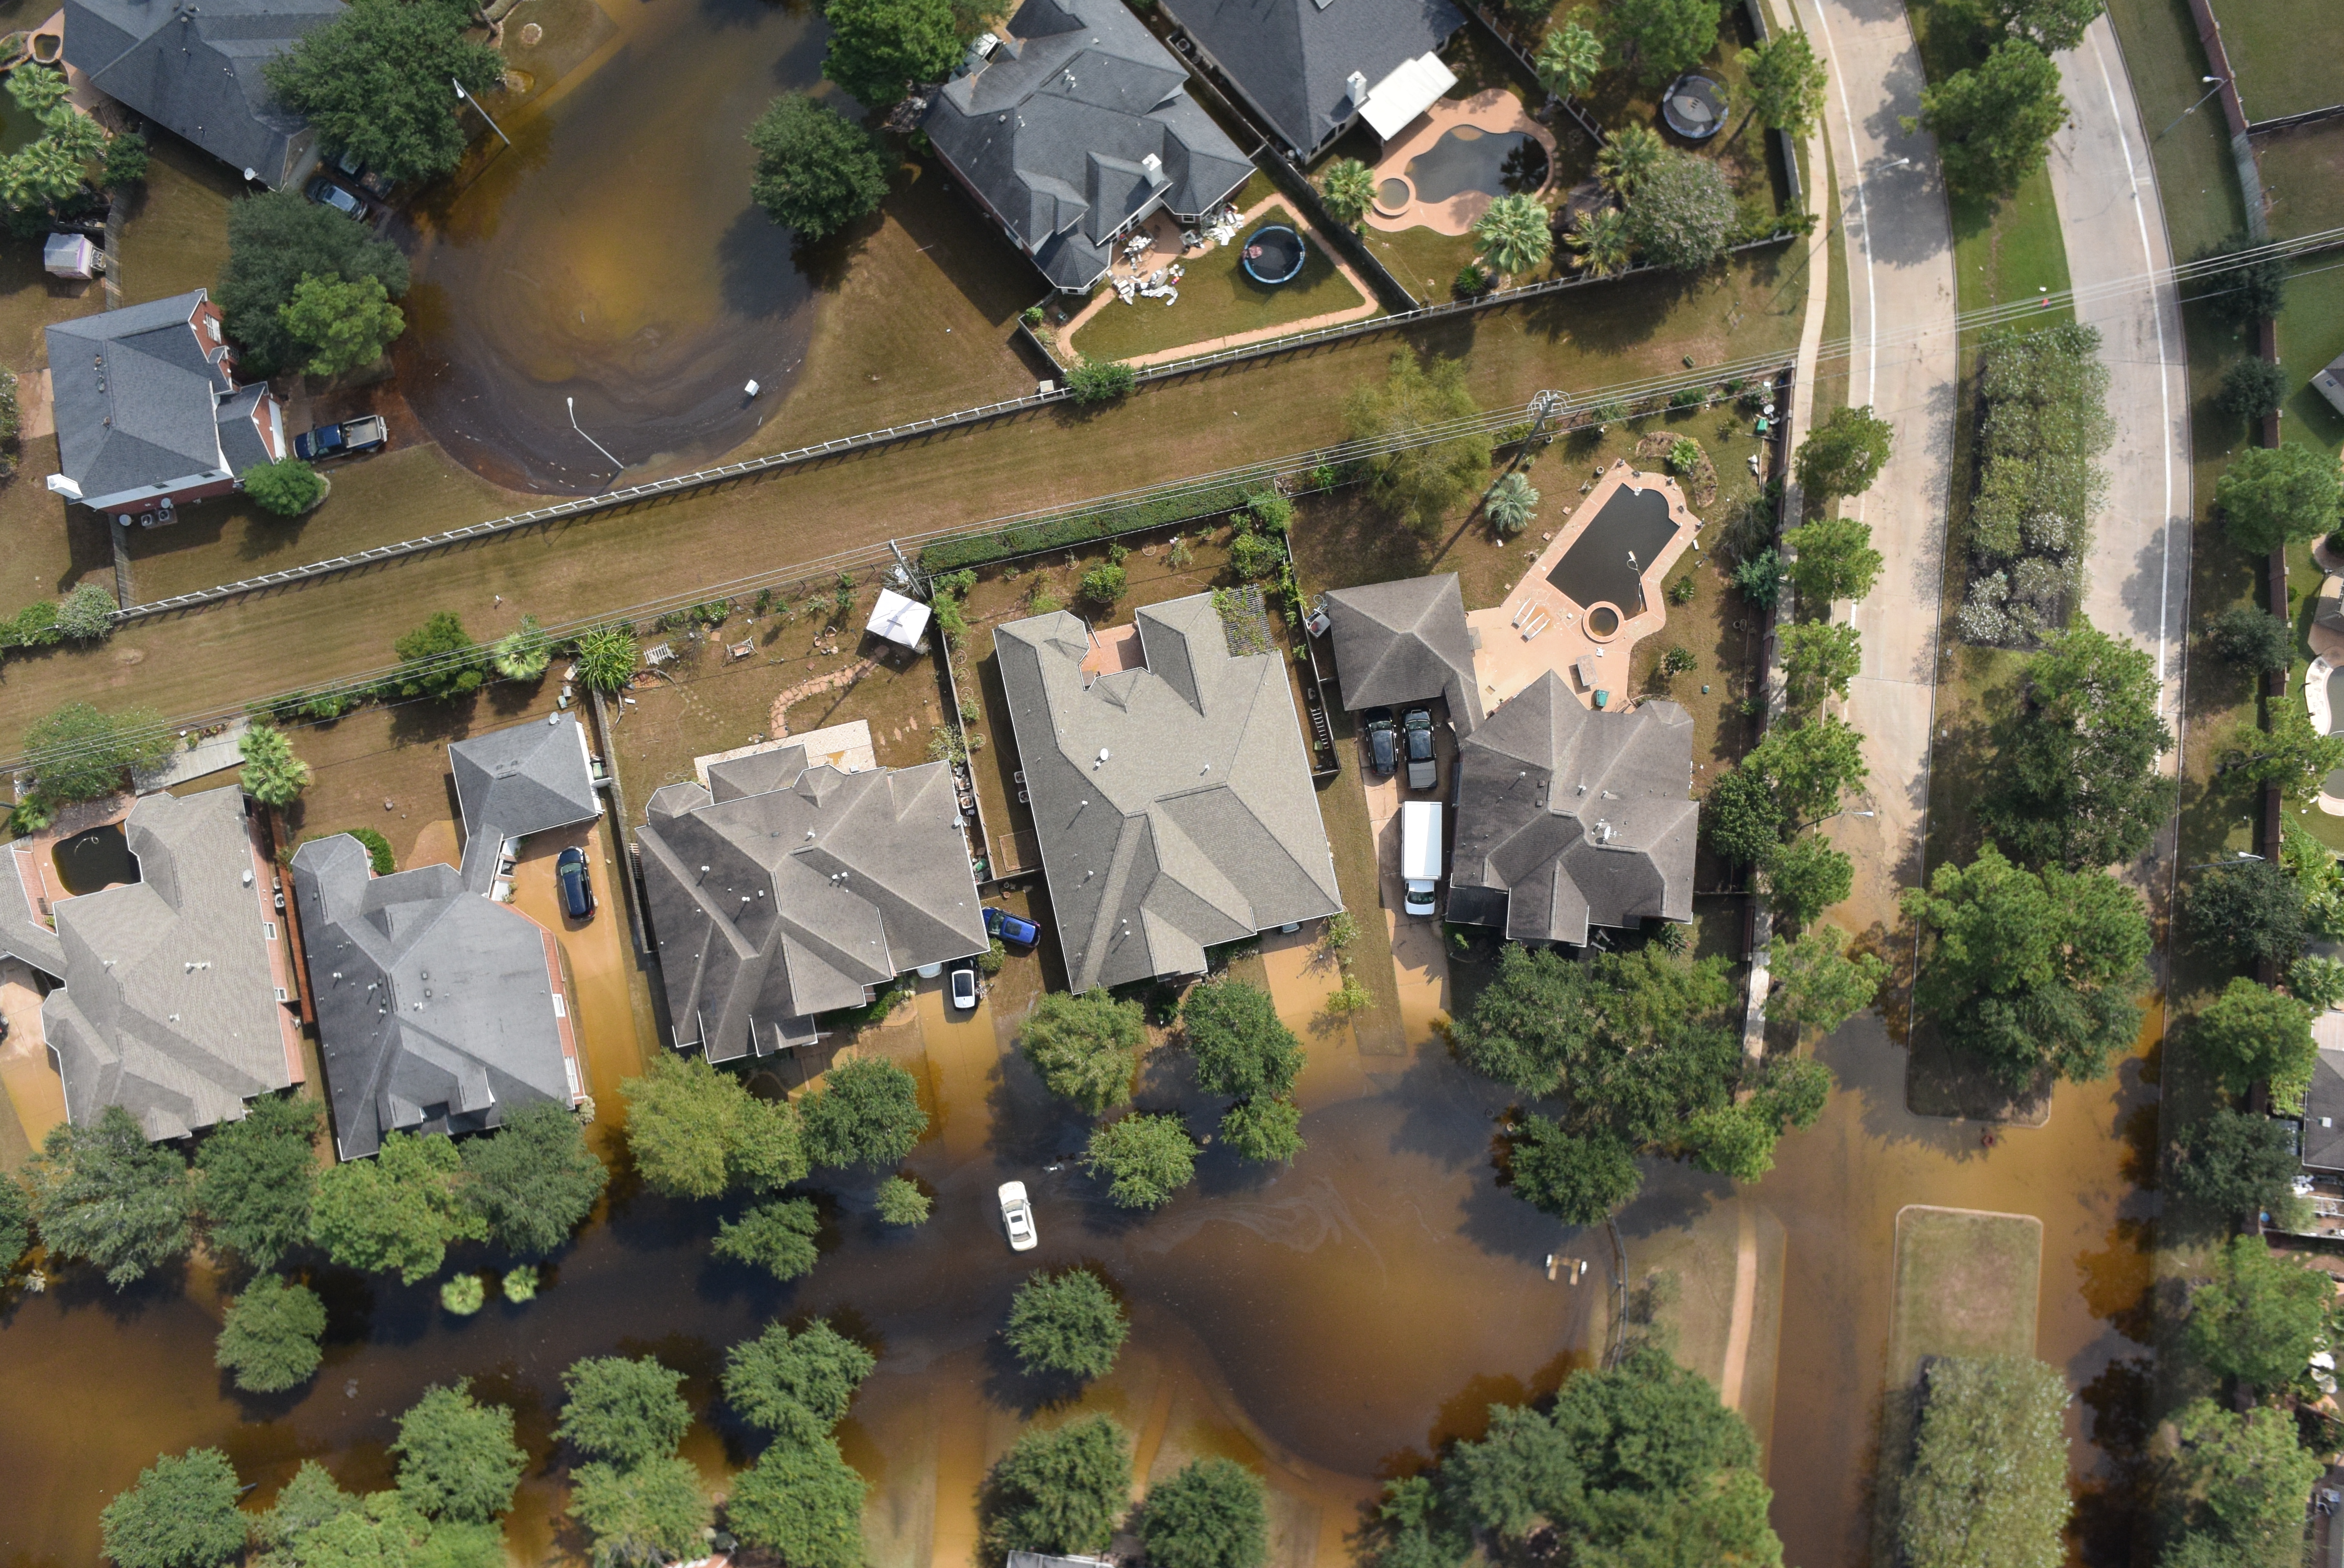
\includegraphics[width=\textwidth]{img/7305.jpg}
         \caption{}
         \label{}
     \end{subfigure}
     \hfill
     \begin{subfigure}[b]{0.45\textwidth}
         \centering
         \includegraphics[width=\textwidth]{img/7305_lab.png}
         \caption{}
         \label{}
     \end{subfigure}
        \caption{Le due figure mostrano un esempio di come una strada allagata può presentare grandi porzioni senza acqua (nella parte in alto a destra), risultando indistinguibile da una strada allagata se non consideriamo il suo contesto.}
        \label{fig:strada_allagata}
    \end{figure}
    
    
    
    \item il dataset al suo interno presenta una grande quantità di rumore, ovvero in alcune maschere sono presenti degli errori. Inoltre, la maggior parte di questi errori sono proprio in immagini che presentano abbondanza di quelle classi menzionate nel punto precedente ("edificio allagato" e "strada allagata"). Di conseguenza, viste già le problematiche menzionate nei punti precedenti, la difficoltà nell'apprenderle aumenta ancora di più. Nello specifico, la maggior parte degli errori trovati nelle maschere del dataset può essere diviso in tre categorie:
    
    \begin{itemize}
        \item la prima tipologia di errore è rappresentata da maschere all'interno delle quali alcuni pixel sono classificati erroneamente. In particolare, i due casi più frequenti sono quelli in cui la classe "strada allagata" oppure la classe "prato" vengono invece classificati come "acqua" (Figura \ref{fig:problem_water}).
        
        \begin{figure}[h!]
         \centering
         \begin{subfigure}[b]{0.45\textwidth}
             \centering
             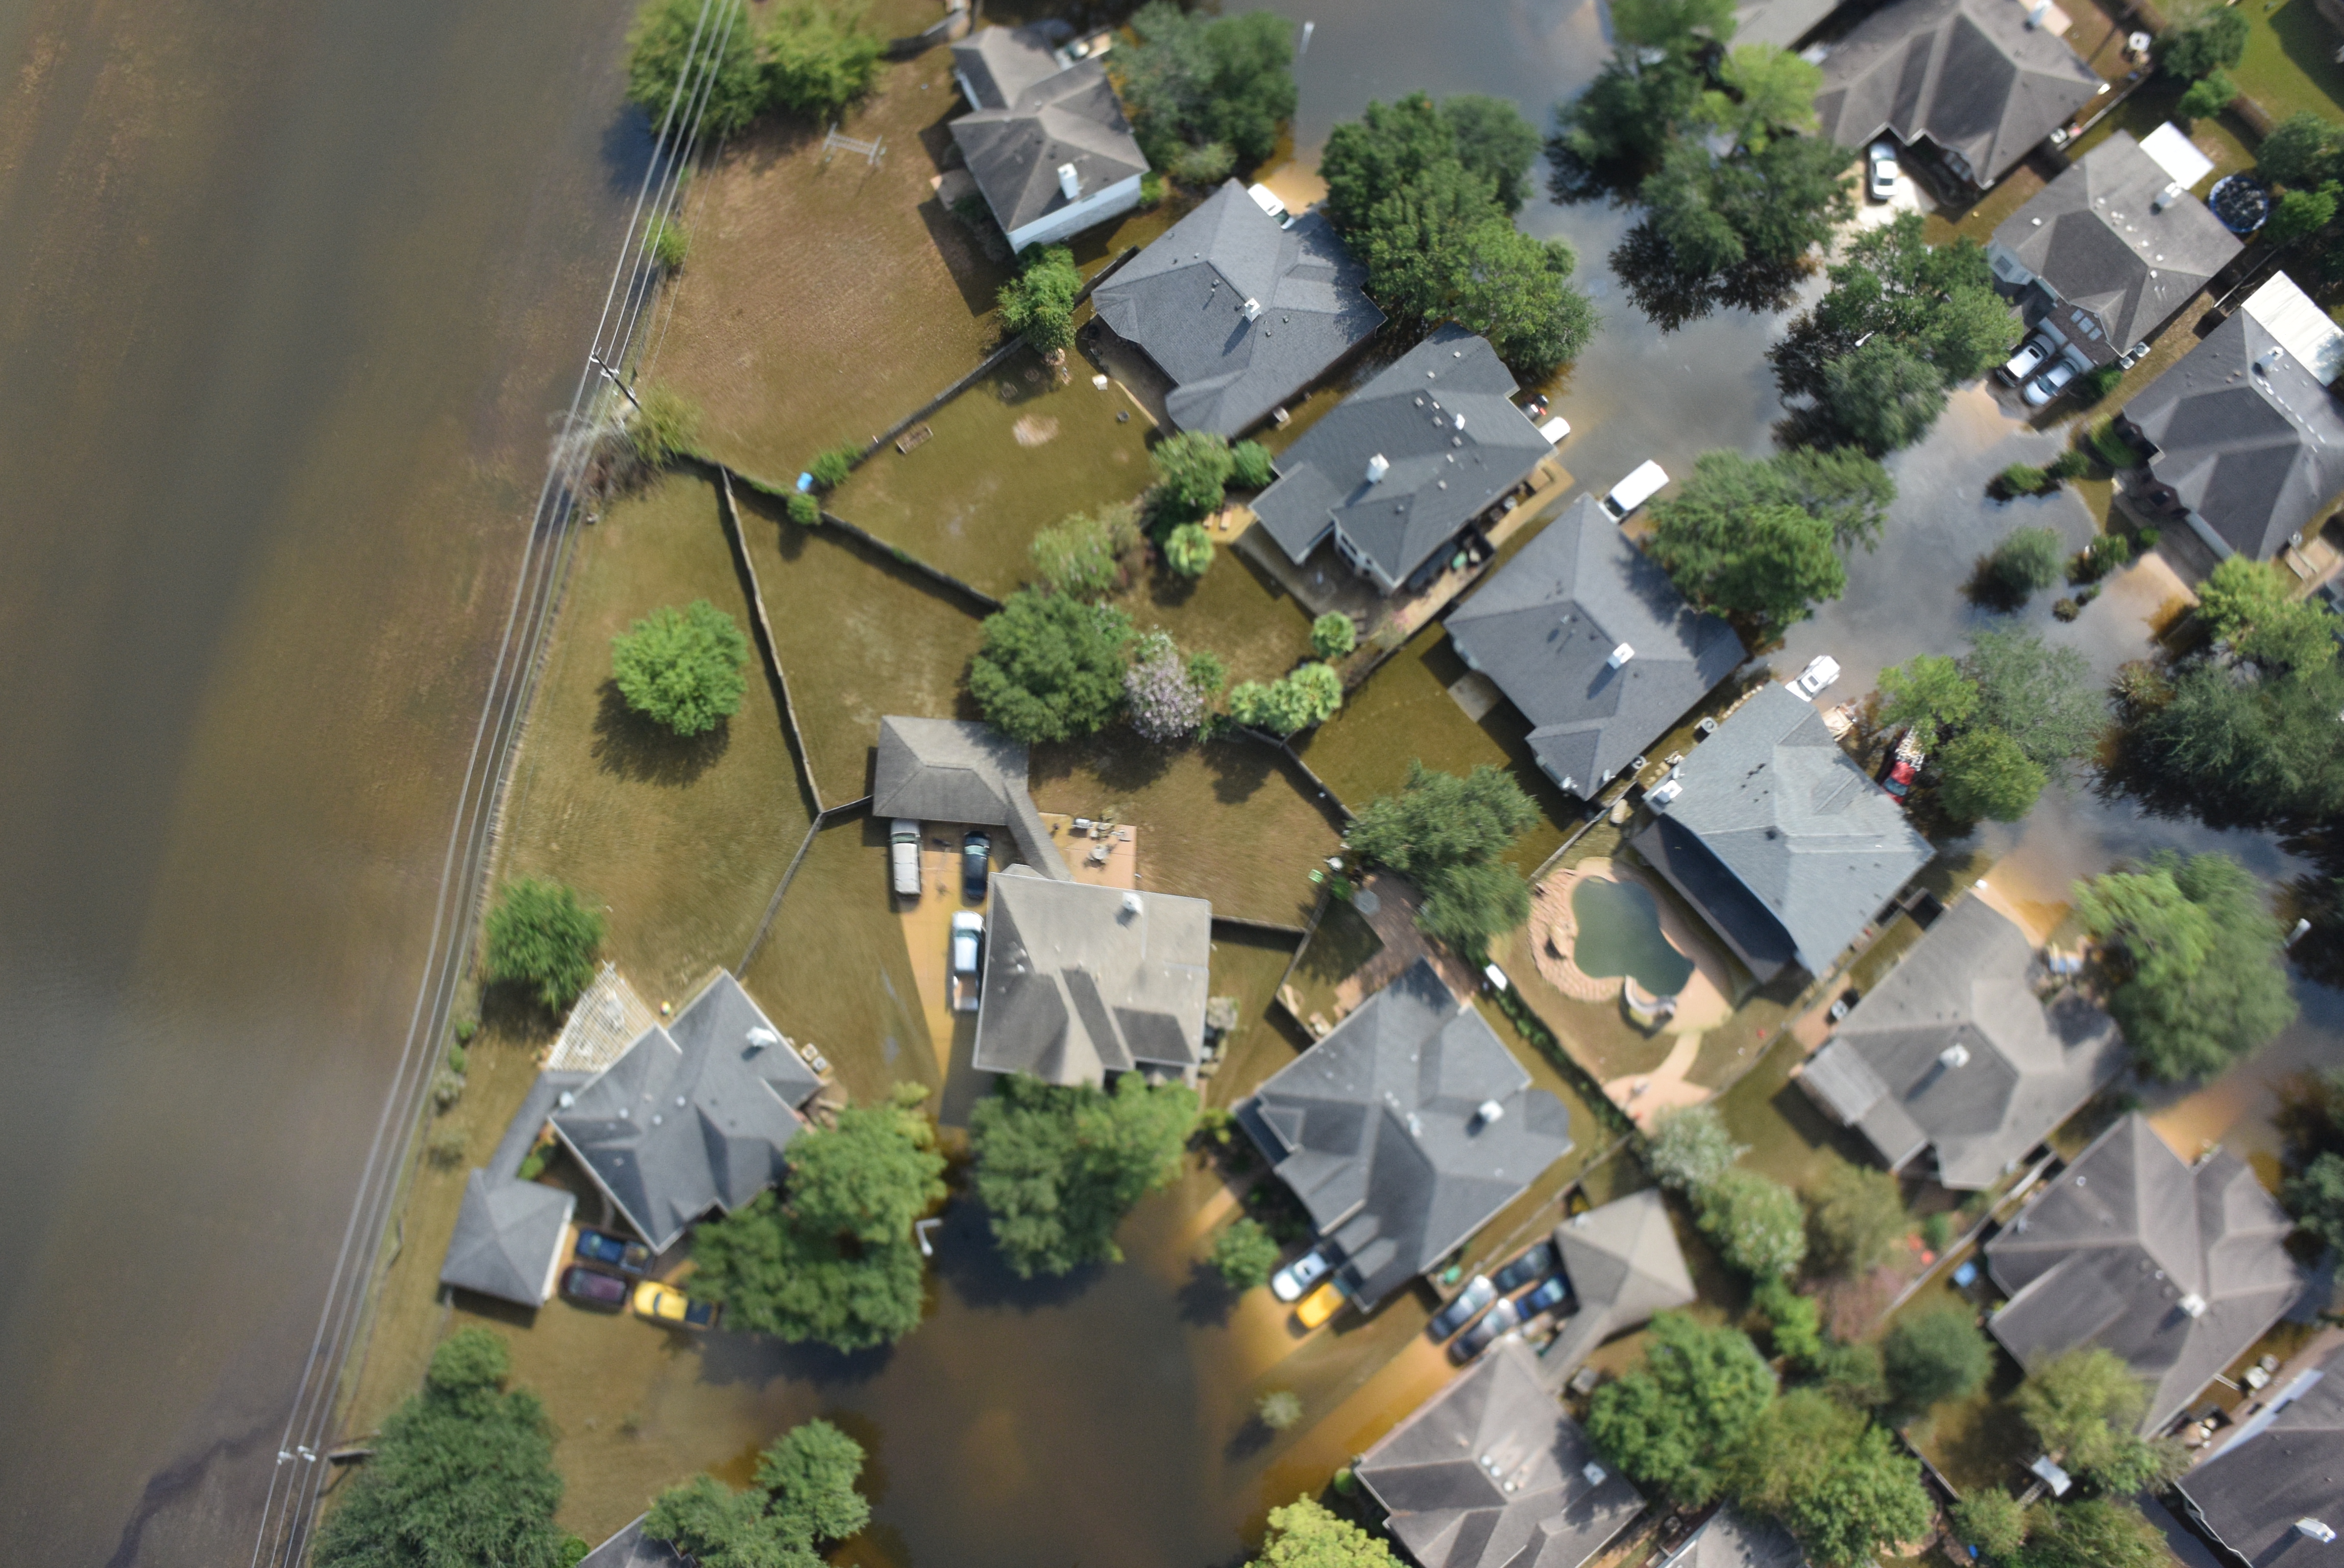
\includegraphics[width=\textwidth]{img/7245.jpg}
             \caption{}
             \label{}
         \end{subfigure}
         \hfill
         \begin{subfigure}[b]{0.45\textwidth}
             \centering
             \includegraphics[width=\textwidth]{img/7245_lab.png}
             \caption{}
             \label{fig:bottleneck}
         \end{subfigure}
            \caption{La figura mostra un esempio di errore presente nel dataset. In particolare, come si può notare i pixel che dovrebbero essere classificati come "prato" vengono invece classificati come "acqua".}
            \label{fig:problem_water}
        \end{figure}
        
        
        
        \item la seconda categoria invece, riguarda quei casi in cui alcune occorrenze di classi o parti di esse non vengono rappresentate nella maschera, ma i corrispettivi pixel vengono invece classificati come appartenti ad altre classi (Figura \ref{fig:problem_water}). I casi più frequenti riguardano le classi "strada" e "strada allagata".
        
        \begin{figure}[h!]
         \centering
         \begin{subfigure}[b]{0.45\textwidth}
             \centering
             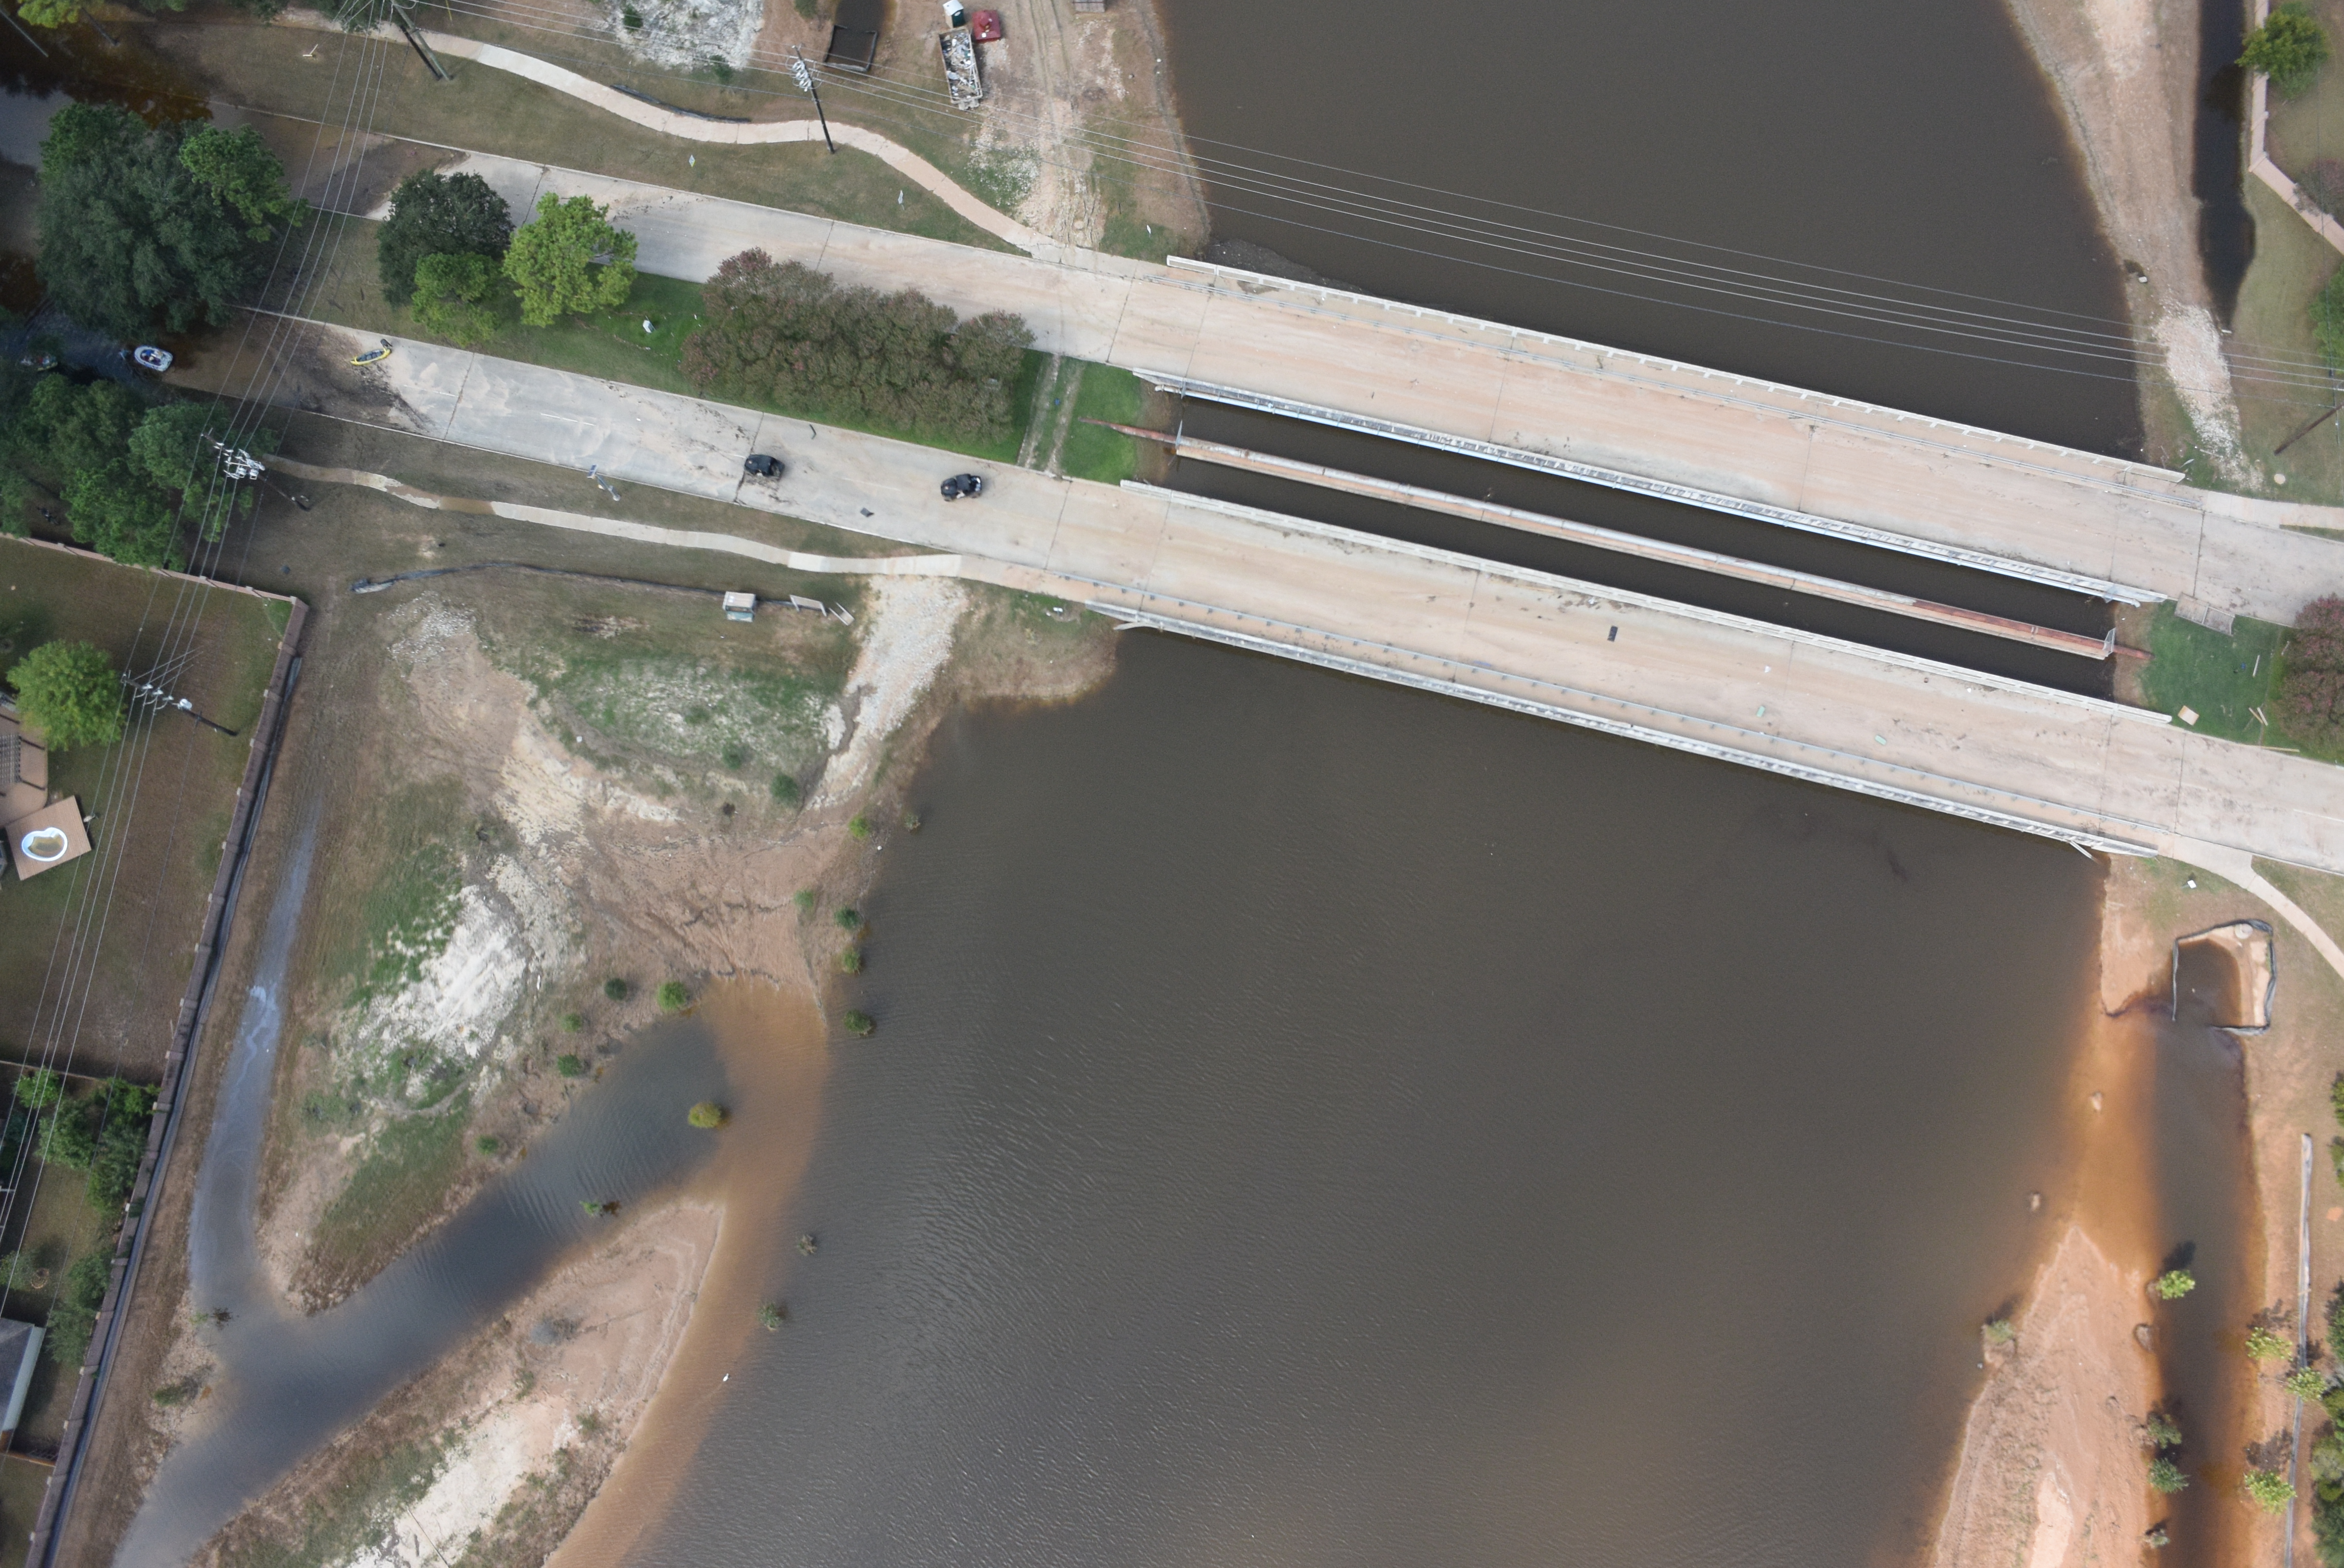
\includegraphics[width=\textwidth]{img/7290.jpg}
             \caption{}
             \label{}
         \end{subfigure}
         \hfill
         \begin{subfigure}[b]{0.45\textwidth}
             \centering
             \includegraphics[width=\textwidth]{img/7290_lab.png}
             \caption{}
             \label{}
         \end{subfigure}
         \hfill
         \begin{subfigure}[b]{0.45\textwidth}
             \centering
             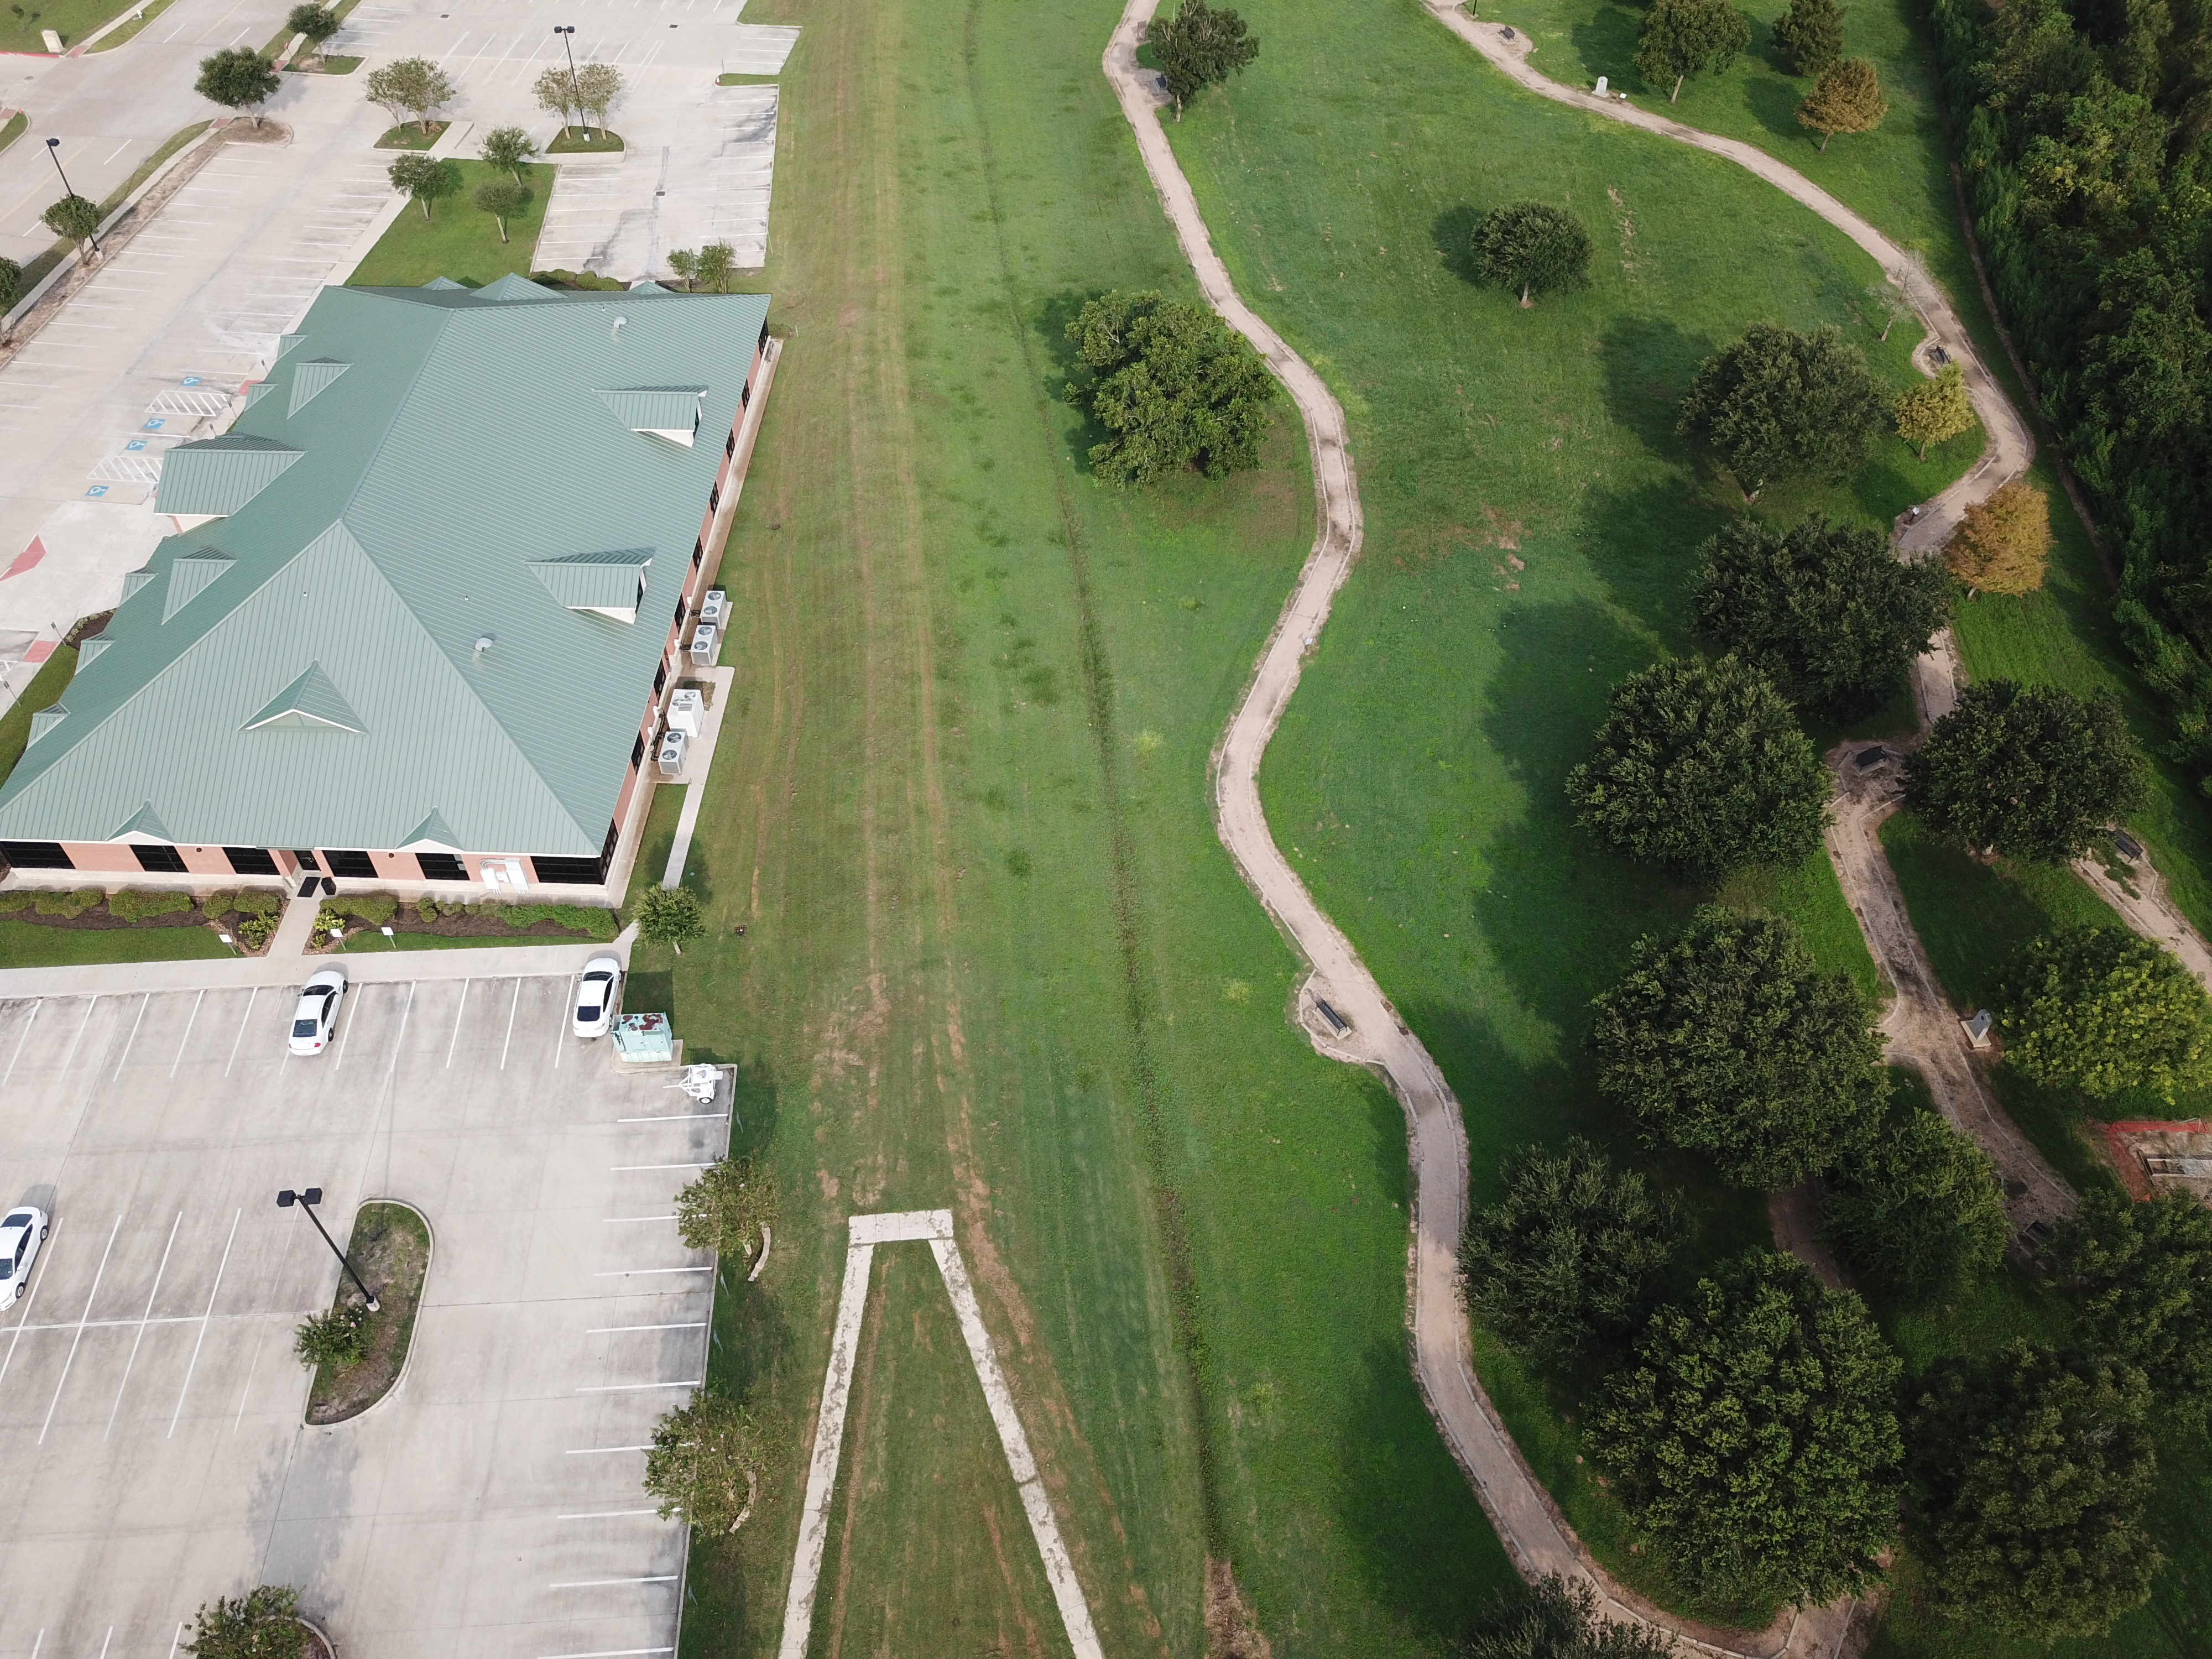
\includegraphics[width=\textwidth]{img/8445.jpg}
             \caption{}
             \label{}
         \end{subfigure}
         \hfill
         \begin{subfigure}[b]{0.45\textwidth}
             \centering
             \includegraphics[width=\textwidth]{img/8445_lab 2.png}
             \caption{}
             \label{}
         \end{subfigure}
            \caption{La figura mostra un esempio della seconda tipologia di errore presente nel dataset. In particolare, come si può notare, nella figura (b) una grossa porzione di un'occorrenza della classe "strada allagata" è mancante e i corrispettivi pixel vengono classificati come "acqua". Nella figura (d) invece un'occorrenza della classe "strada" non viene segnalata e i corrispettivi pixel vengono classificati come "prato".}
            \label{fig:problem_water}
        \end{figure}
        
        
        \item il terzo caso riguarda invece, la presenza di porzioni d'immagine fortemente incoerenti tra loro, oltre che con un certo grado di "confusione" tra le classi. La Figura \ref{fig:problem_confusion} ne illustra un esempio. 
        
        
        \begin{figure}[h!]
         \centering
         \begin{subfigure}[b]{0.45\textwidth}
             \centering
             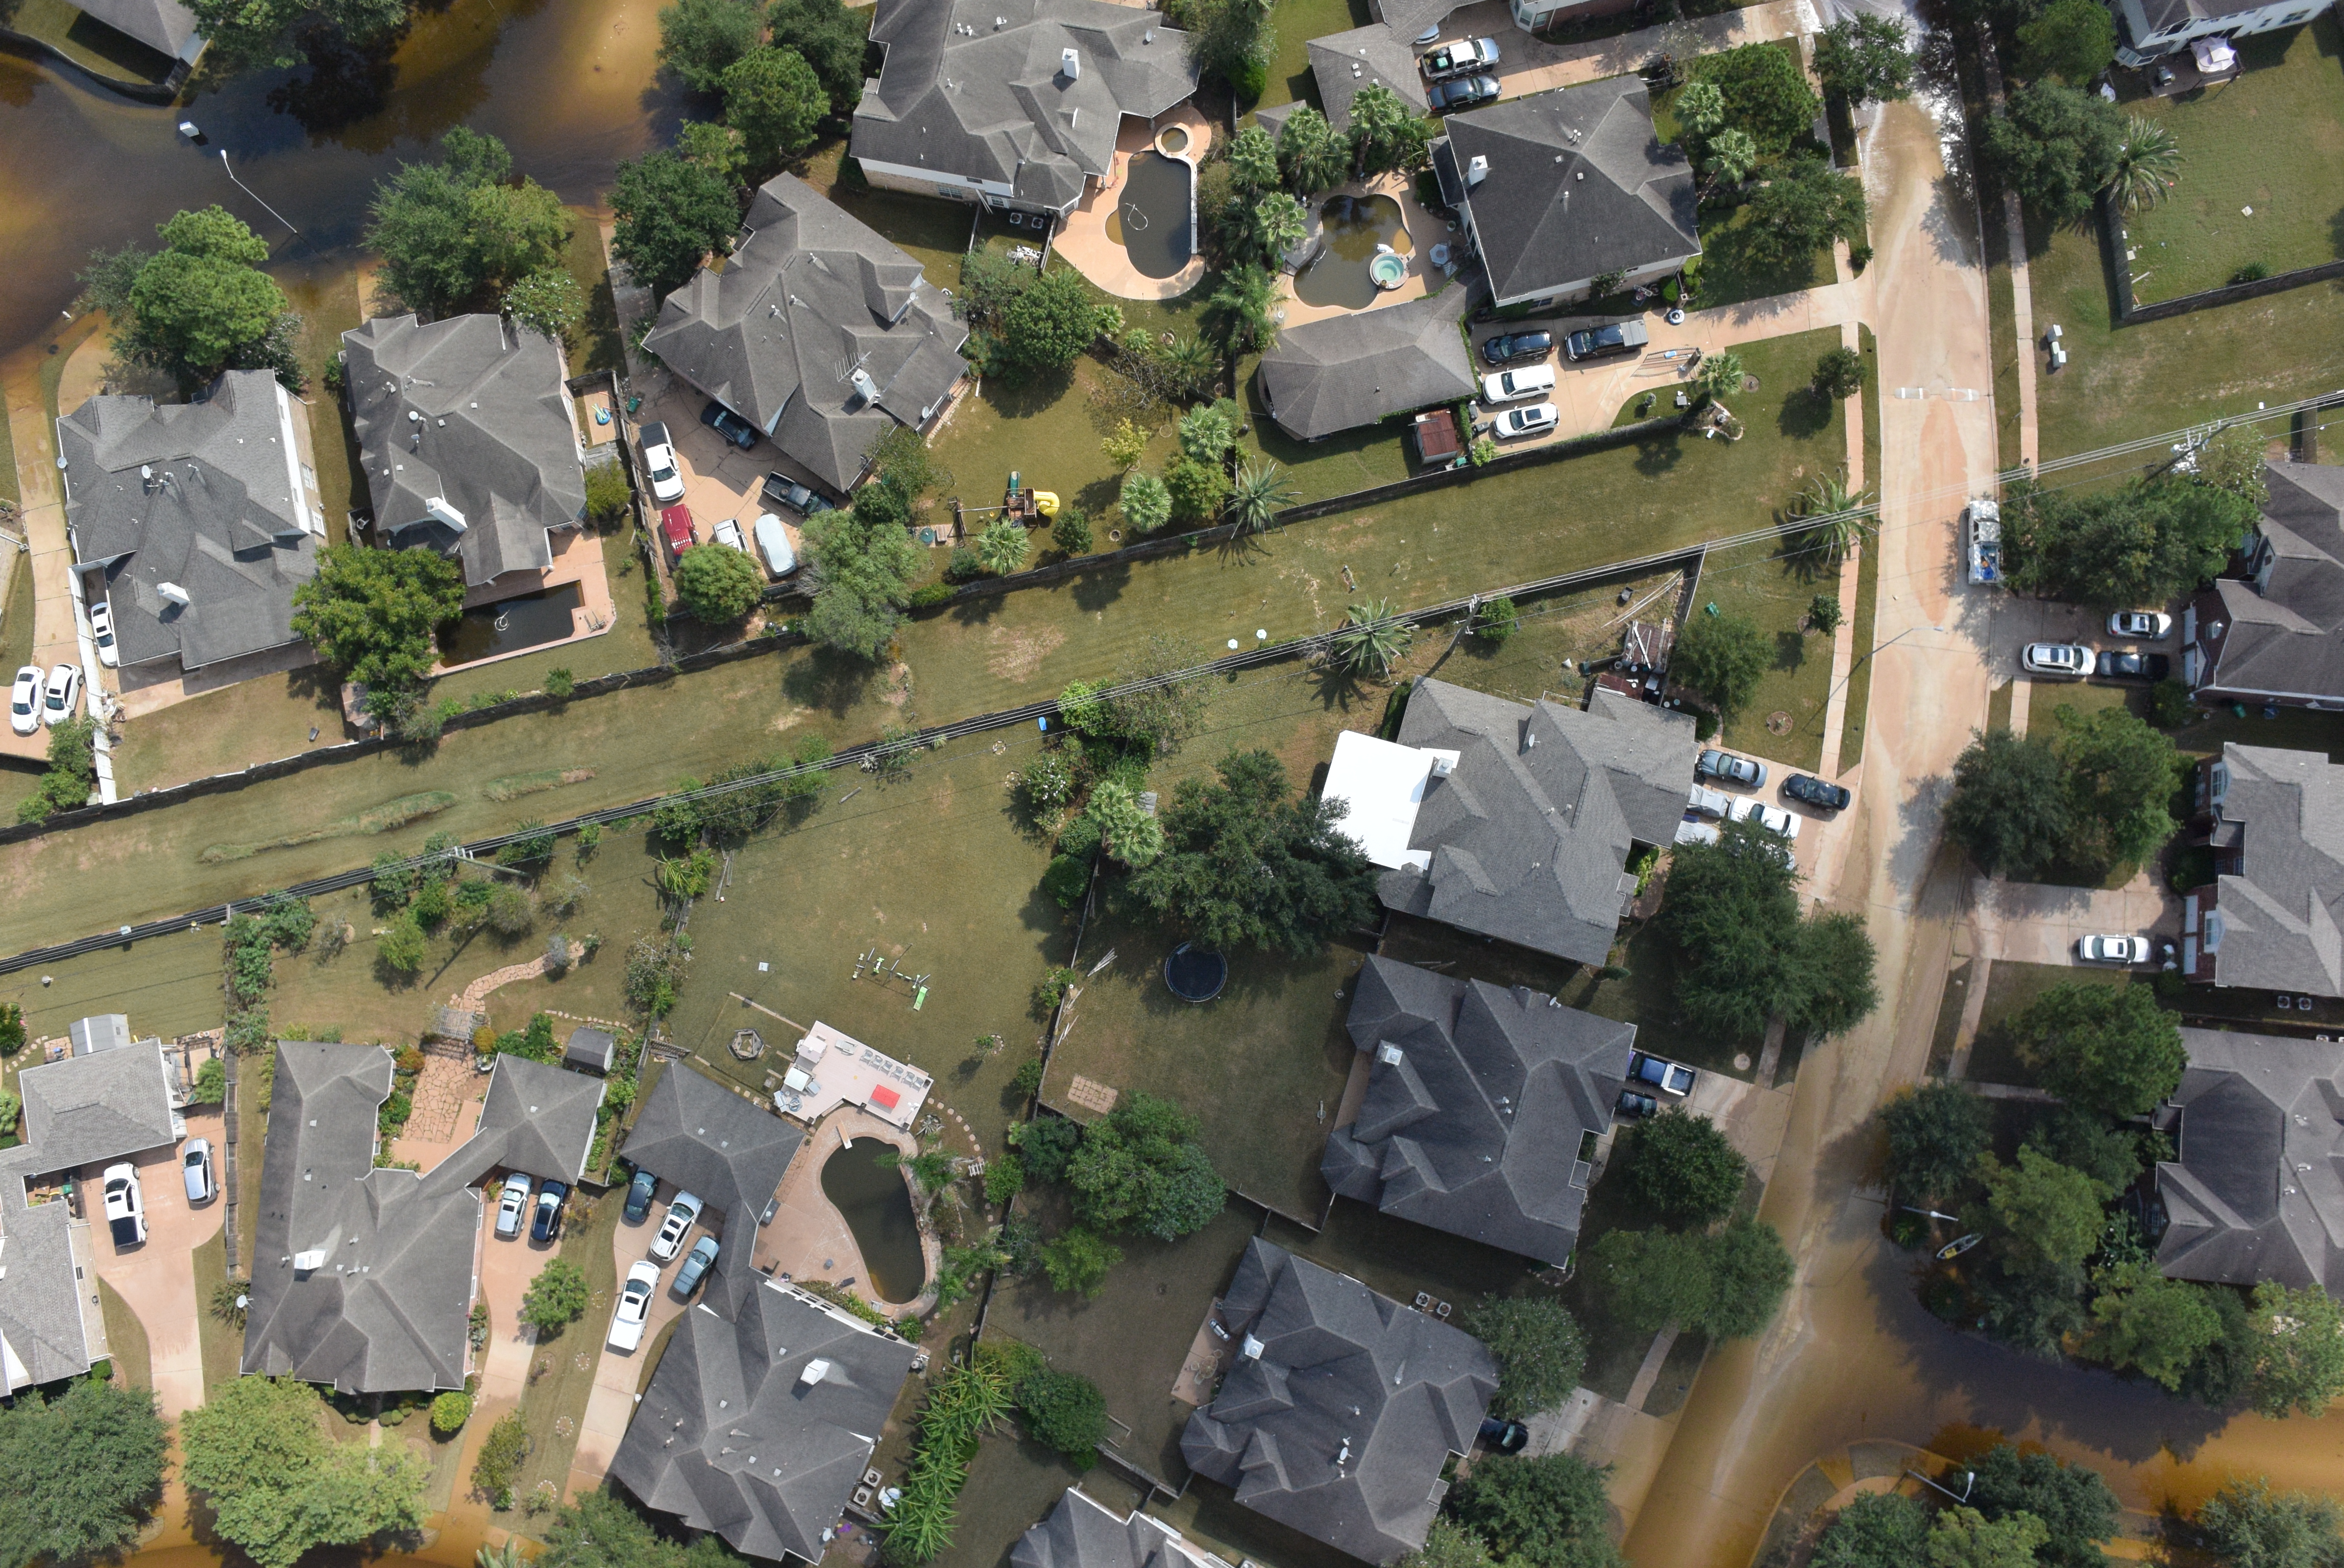
\includegraphics[width=\textwidth]{img/7614.jpg}
             \caption{}
             \label{}
         \end{subfigure}
         \hfill
         \begin{subfigure}[b]{0.45\textwidth}
             \centering
             \includegraphics[width=\textwidth]{img/7614_lab 2.png}
             \caption{}
             \label{}
         \end{subfigure}
            \caption{La figura mostra un esempio della terza tipologia di errore presente nel dataset. In particolare, come si può notare, nella parte destra della maschera c'è un incoerenza rappresentata dal fatto che porzioni diverse della stessa strada vengono classificate come "strada non allagata" e "strada allagata", anche se vi è presenza di acqua. Inoltre, alcuni edifici circondati da strade allagate vengono classificati come "edificio non allagato". Infine, nella parte centrale dell'immagine viene segnalata un'occorrenza della classe "strada non allagata", quando in realtà nell'immagine non risulta.}
            \label{fig:problem_confusion}
        \end{figure}
        
    \end{itemize}
    
\end{itemize}










\section{Pulizia del dataset e Data Augmentation}
\label{data_aug_used}
Per far fronte a due delle quattro principali difficoltà menzionate nel paragrafo precedente, si sono messe in atto due fasi principali di pulizia del dataset (\textit{data cleaning}) e di data augmentation offline.
In particolare, queste due fasi sono risultate fondamentali per fornire un dataset composto da immagini elevate sia da un punto di vista qualitativo che quantitativo, fattore in generale  indispensabile per addestrare una rete neurale.
Partendo dalla pulizia del dataset, che è servita soprattutto ad ovviare al problema della presenza degli errori, questa fase è stata lunga e articolata, in quanto è stata effettuata una scansione manuale, confontando ogni immagine del dataset con la sua maschera corrispondente, al fine di individuare eventuali errori. Da questa scansione, si è riscontrato che in totale 182 immagini presentavano errori importanti, come quelli descritti nel paragrafo precedente. Di queste 182, ben 160 erano immagini contenenti entrambe le classi "allagate" (strada ed edificio). Confrontando quest'ultimo dato con il numero totale di immagini contenente queste due classi (all'incirca 200), si può notare come, oltre alle difficoltà intrinseche delle due classi, questa notevole presenza di errori le abbia fortemente svantaggiate. In seguito a questa fase di accertamento della consistenza del problema, si è proseguito con la fase di correzione. Durante questa fase, una parte degli errori è risultata corregibile attraverso diversi metodi, a seconda della natura dell'errore, altri invece, a causa della loro natura non hanno permesso la correzione in tempi non troppo lunghi e di conseguenza, per non rallentare troppo il lavoro, sono state scartate. In particolare, delle 182 totali, 45  non state corrette ma scartate. La Figura \ref{fig:esempio_correzioni} mostra un esempio di come una maschera contenente un errore sia stata corretta.
\\


\begin{figure}[h!]
    \centering
    \begin{subfigure}[b]{0.6\textwidth}
        \centering
        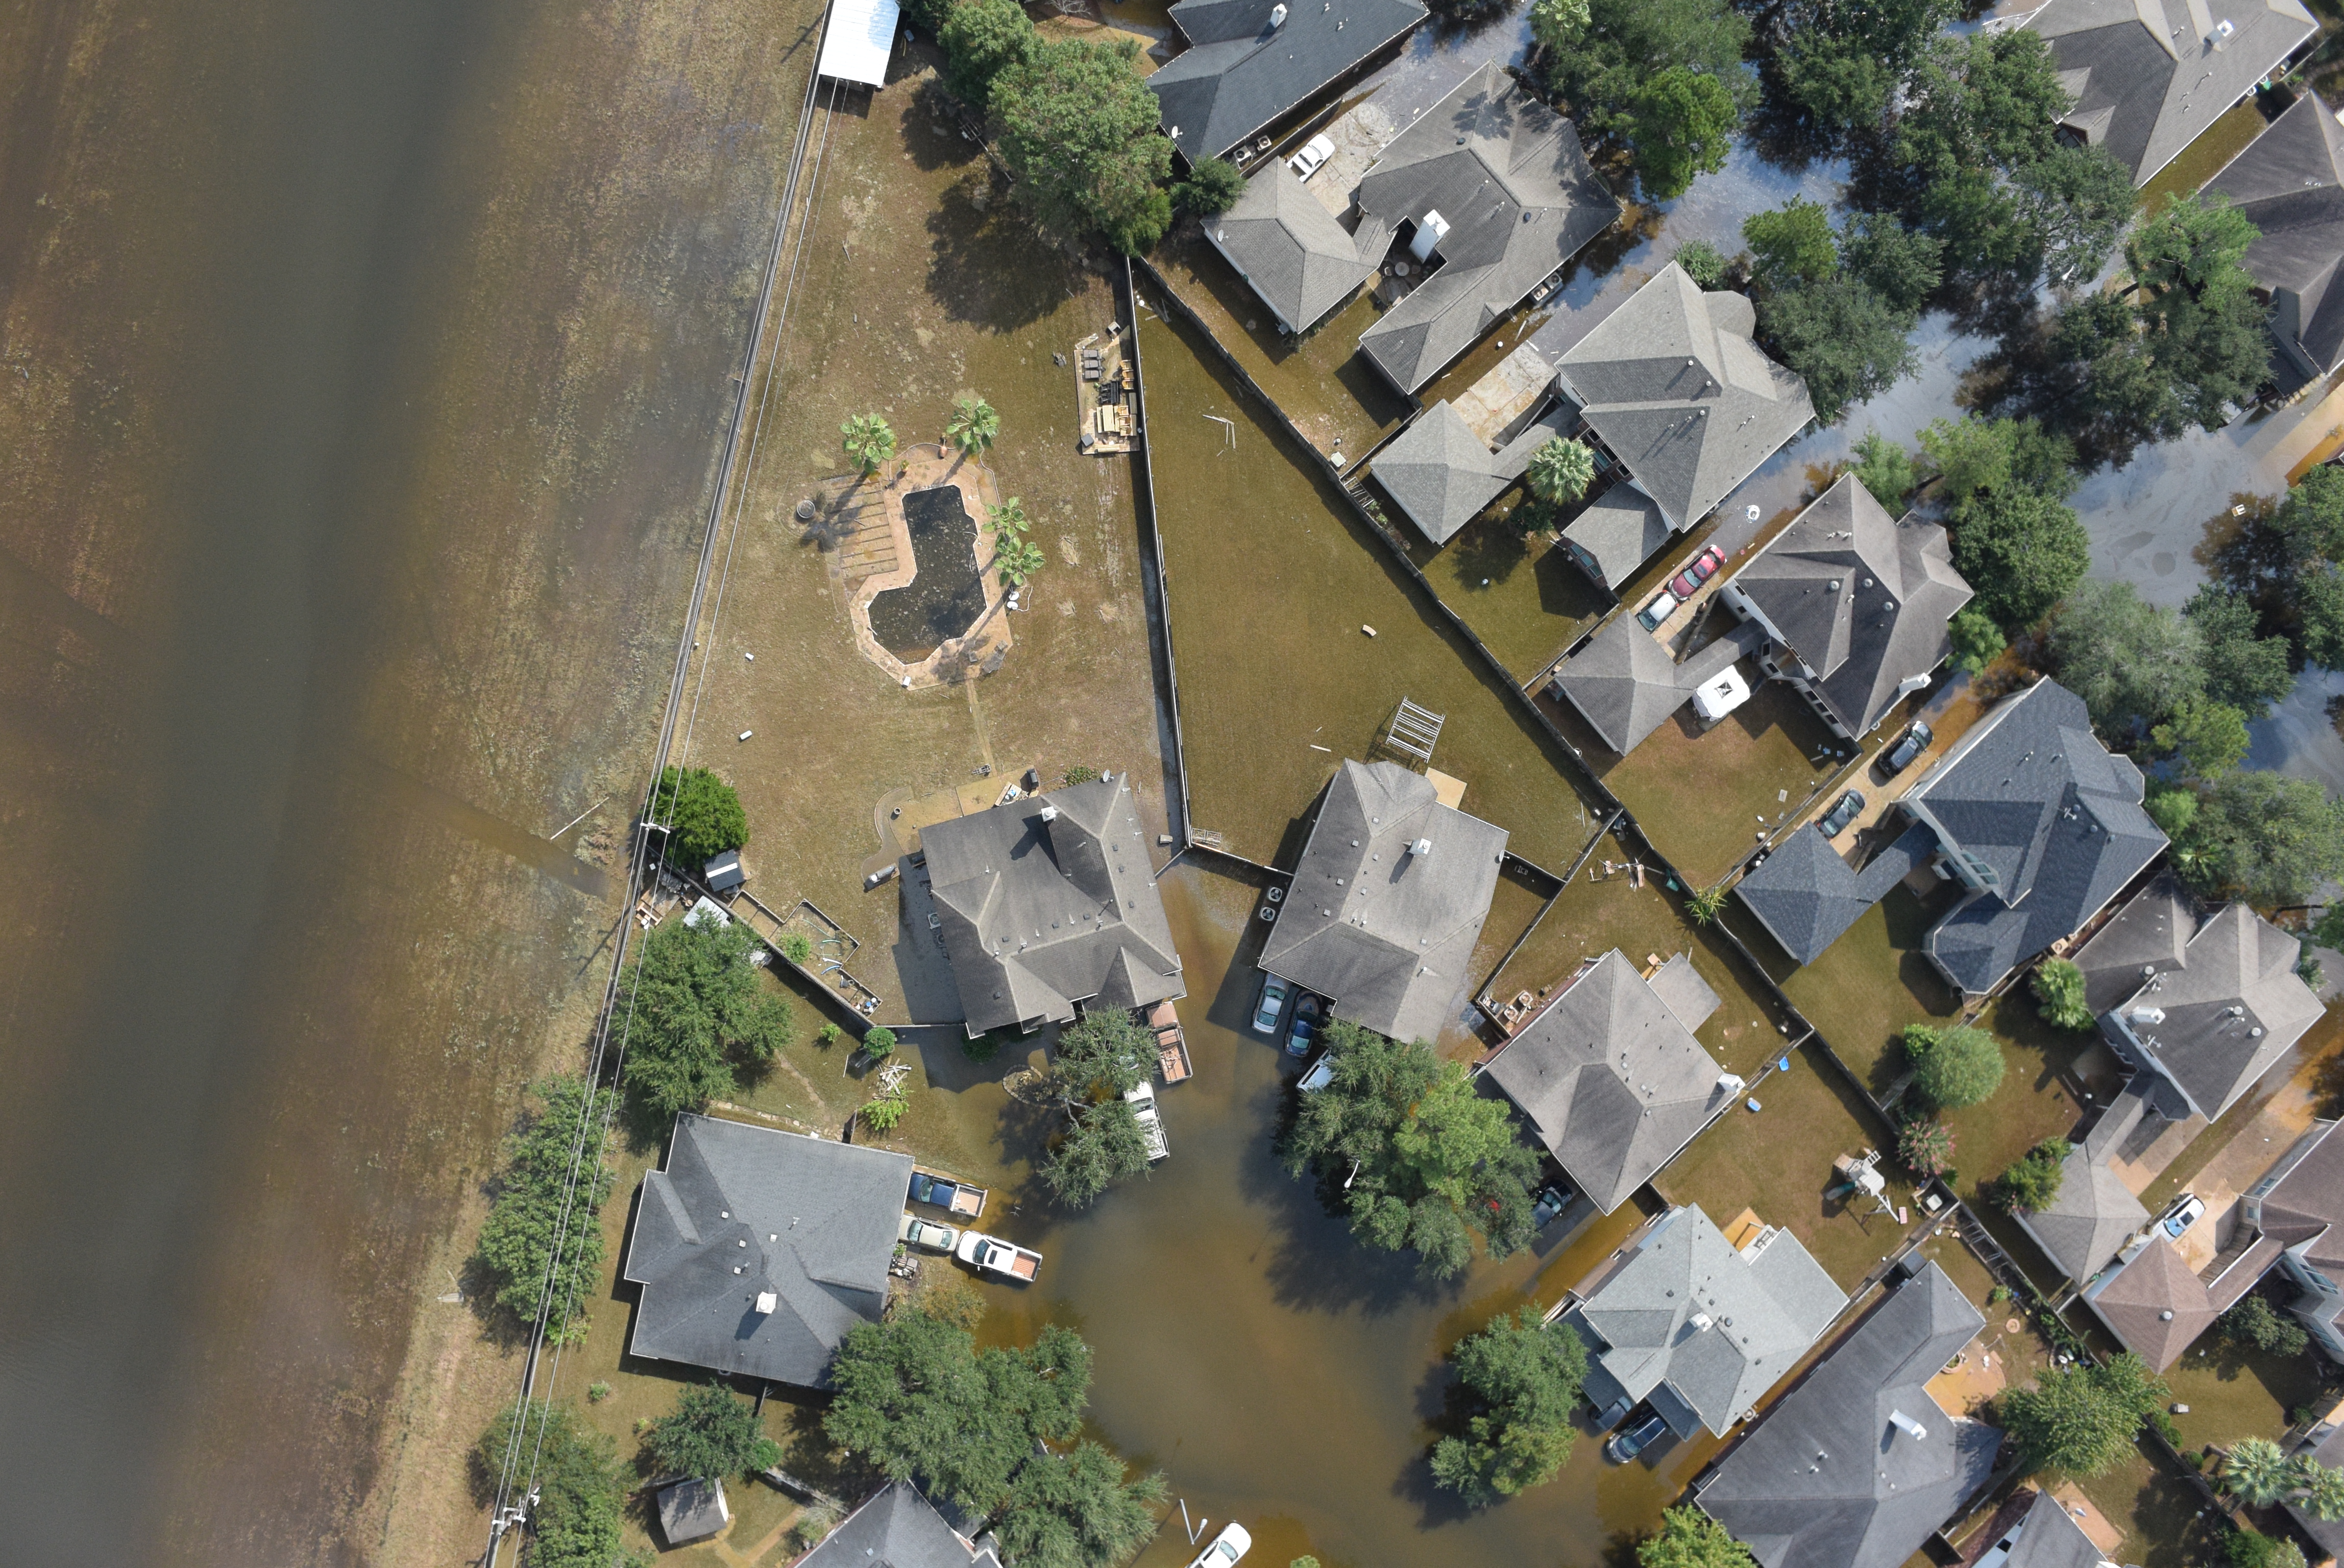
\includegraphics[width=\textwidth]{img/7252.jpg}
        \caption{}
        \label{}
    \end{subfigure}
    \hfill
    \begin{subfigure}[b]{0.45\textwidth}
        \centering
        \includegraphics[width=\textwidth]{img/7252_lab.png}
        \caption{}
        \label{}
    \end{subfigure}
    \hfill
    \begin{subfigure}[b]{0.45\textwidth}
        \centering
        \includegraphics[width=\textwidth]{img/7252_lab 2.png}
        \caption{}
        \label{}
    \end{subfigure}
    \caption{Le tre figure sono un esempio di correzione fatto sulle maschere del dataset FloodNet. La figura (a) è l'immagine a cui si riferiscono le due maschere (b) e (c). Come si può notare, nella (b) una porzione di prato è invece classificata come acqua (celeste), mentre la (c) è la versione corretta.}
    \label{fig:esempio_correzioni}
\end{figure}

Mentre la fase di pulizia ha cercato di ovviare soprattutto alla quarta problematica, la fase successiva di data augmentation offline ha invece cercato di risolvere soprattutto la problematica dello sbilanciamento verso alcune classi.

Come evidenziato dagli autori di \cite{data_aug_effects}, la data augmentation può creare degli effetti indesiderati, svantaggiando una classe rispetto ad altre. Per questo motivo, questa fase di data augmentation offline non è stata fatta su tutto il dataset, ma su un gruppo di immagini selezionate. In particolare, come già detto, lo scopo della selezione è stato di aumentare la presenza di quelle classi che riguardano la problematica dello sbilanciamento, specialmente le classi "strada allagata" e "edificio allagato", senza però sbilanciare ancora di più il dataset verso classi molto presenti, come la classe "prato". 
Per l'implementazione di questa data augmentation è stata utilizzata la nota libreria Albumentations \cite{albumentations} e il meccanismo generale è stato il seguente: ad ognuna delle 140 immagini selezionate è stata applicata per tre volte una combinazione randomica di quattro operazioni (non sempre tutte e quattro), producendo  per ogni immagine ulteriori tre (Figura \ref{fig:esempi_data_aug}). In particolare, le trasformazioni utilizzate sono: \textit{Rotate}, che consiste nella rotazione di una quantità randomica di gradi dell'immagine; \textit{VerticalFlip}, ovvero l'immagine viene ruotata su sé stessa sull'asse che la attraversa orizzontalmente; \textit{HorizontalFlip}, ovvero la stessa trasformazione ma sull'asse verticale; e infine \textit{RandomBrightnessContrast}, che consiste nell'alterare randomicamente la luminosità e il contrasto dell'immagine.

\begin{figure}[h!]
     \centering
     \begin{subfigure}[b]{0.45\textwidth}
         \centering
         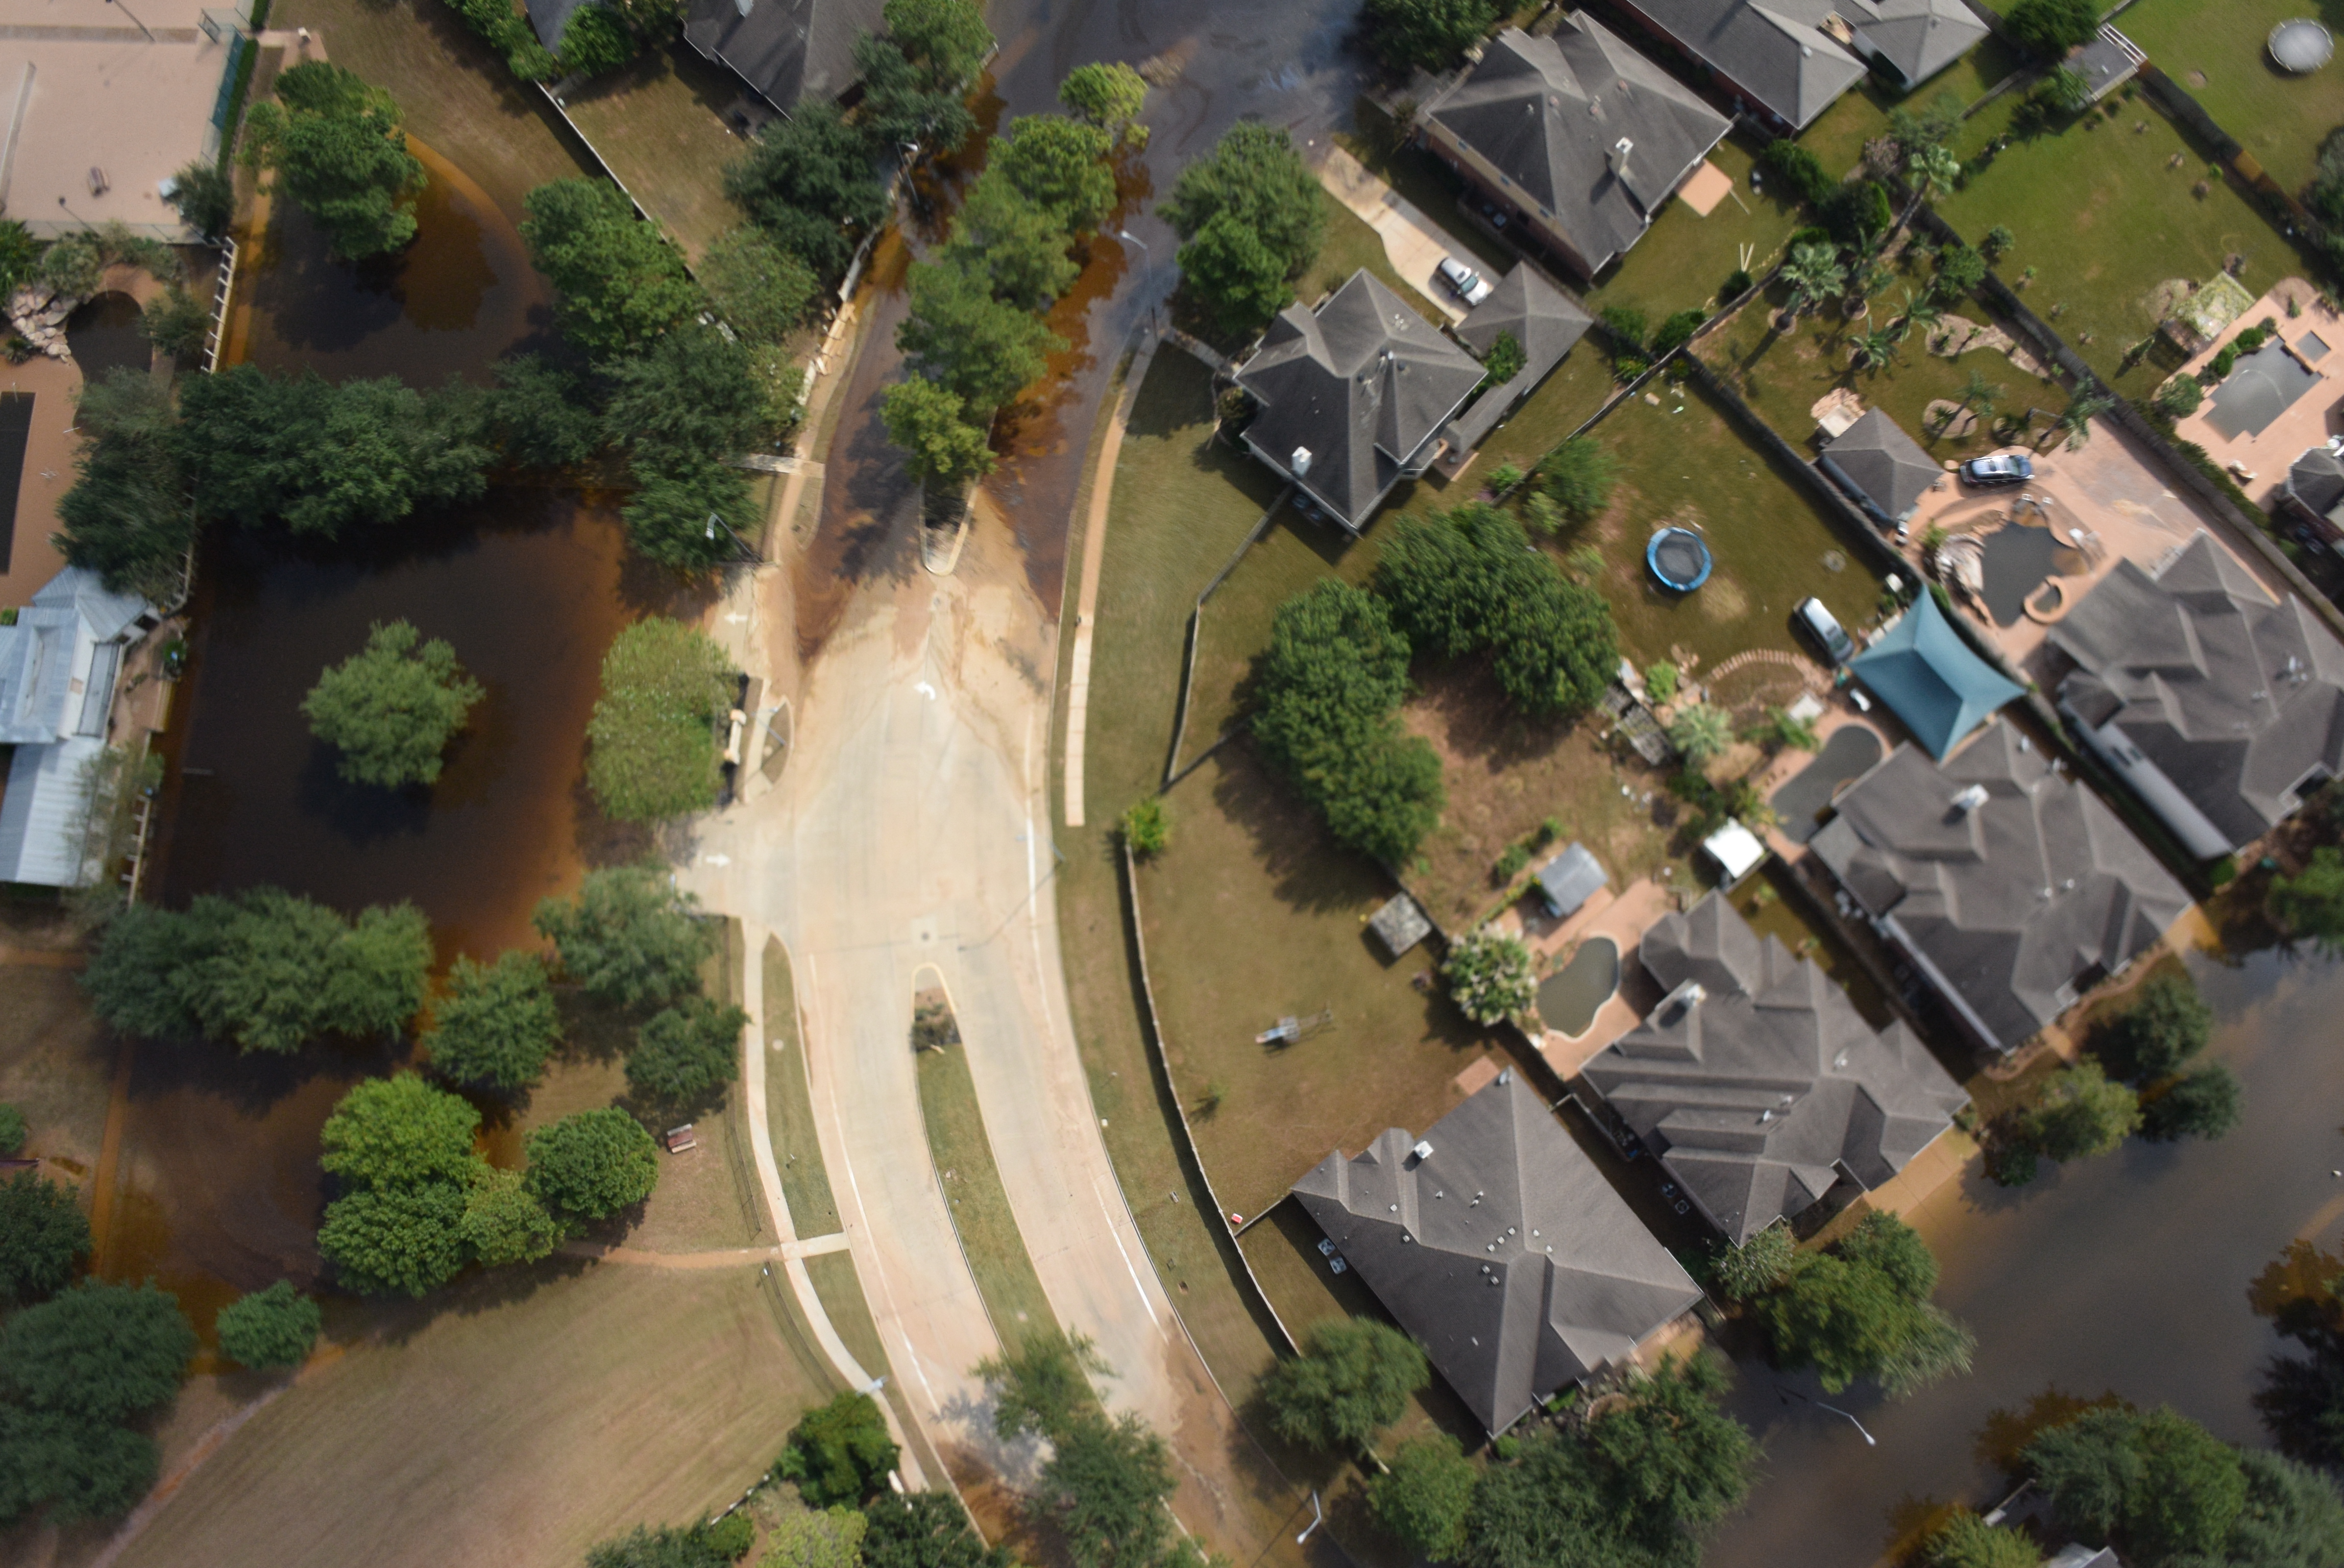
\includegraphics[width=\textwidth]{img/7310.jpg}
         \caption{}
         \label{}
     \end{subfigure}
     \hfill
     \begin{subfigure}[b]{0.45\textwidth}
         \centering
         \includegraphics[width=\textwidth]{img/7310_lab.png}
         \caption{}
         \label{}
     \end{subfigure}
     \hfill
     \begin{subfigure}[b]{0.45\textwidth}
         \centering
         \includegraphics[width=\textwidth]{img/7310_0.jpg}
         \caption{}
         \label{}
     \end{subfigure}
     \hfill
     \begin{subfigure}[b]{0.45\textwidth}
         \centering
         \includegraphics[width=\textwidth]{img/7310_0_lab.png}
         \caption{}
         \label{}
     \end{subfigure}
     \hfill
     \begin{subfigure}[b]{0.45\textwidth}
         \centering
         \includegraphics[width=\textwidth]{img/7310_1.jpg}
         \caption{}
         \label{}
     \end{subfigure}
     \hfill
     \begin{subfigure}[b]{0.45\textwidth}
         \centering
         \includegraphics[width=\textwidth]{img/7310_1_lab.png}
         \caption{}
         \label{}
     \end{subfigure}
     \begin{subfigure}[b]{0.45\textwidth}
         \centering
         \includegraphics[width=\textwidth]{img/7310_2.jpg}
         \caption{}
         \label{}
     \end{subfigure}
     \hfill
     \begin{subfigure}[b]{0.45\textwidth}
         \centering
         \includegraphics[width=\textwidth]{img/7310_2_lab.png}
         \caption{}
         \label{}
     \end{subfigure}
     
        \caption{Le otto figure mostrano un esempio della data augmentation utilizzata offline prima dell'addestramento. Le figure (a) e (b) sono l'immagine e la maschera originali, mentre tutte le altre sono il risultato dell'applicazione di un sottoinsieme delle operazioni Rotate, HorizontalFip, VerticalFlip e RandomBrightnessContrast.}
        \label{fig:esempi_data_aug}
\end{figure}

 Oltre ad utilizzare la data augmentation offline, per aumentare il numero di immagini del dataset ed ovviare al problema dello sbilanciamento, è stata utilizzata una seconda fase di data augmentation online, ovvero durante l'addestramento. Lo scopo, in questo caso, non era aumentare il numero di immagini ma ottenere un effetto regolarizzante apportando ad ogni epoca dell'addestramento una diversa modifica ad ogni immagine. L'intuizione dietro questo metodo è che in questo modo, ad ogni epoca il modello vede una versione del dataset leggermente diversa e questo evita che andando avanti nell'addestramento il modello cada nel meccanismo di overfitting. In particolare, anche qui per l'implementazione è stata utilizzata la libreria Albumentations e il meccanismo generale è il seguente: durante un'epoca, ad ogni caricamento di un'immagine per la costruzione di una batch viene applicata un'operazione di \textit{VerticalFlip}, una di \textit{HorizontalFlip} e infine una di \textit{RandomBrightnessContrast}. La chiave di questo metodo è che, come nella data augmentation fatta offline, ad ogni trasformazione viene associata una probabilità, di conseguenza ad ogni epoca non vengono applicate tutte e tre le trasformazioni, ma solo un sottoinsieme randomico delle tre, creando nella pratica una versione diversa del dataset ad ogni epoca.














\section{DeepLabV3}
\label{paragr_deeplabv3}
Le principali difficoltà che gli autori di \cite{deeplabv1, deeplabv2, deeplabv3} hanno evidenziato riguardo l'applicazione delle DCNN al task generale della segmentazione semantica sono due: la prima si riferisce alla bassa risoluzione delle feature map prodotte dalle DCNN, mentre la seconda riguarda la presenza all'interno dell'immagine di oggetti a diversa scala. In particolare, soprattutto la seconda difficoltà presenta un forte parallelo con una delle principali problematiche affrontate in questo lavoro. Ed è proprio questa la motivazione per cui si è scelto di utilizzare questo modello. Riprendendo il discorso delle difficoltà delle DCNN nella segmentazione semantica, la prima difficoltà è soprattutto causata dalla combinazione e dall'alternarsi di strati di pooling e convoluzioni con stride. In particolare, questa è una caratteristica che rappresenta uno dei punti di forza delle DCNN in campi come la classificazione, dove ridurre la risoluzione delle feature map serve proprio ad apprendere rappresentazioni molto astratte del dato e ad acquisire l'invarianza rispetto a sue trasformazioni locali. Chiaramente, questo punto di forza si trasforma in una debolezza nel task della segmentazione, in cui la localizzazione è fondamentale. La seconda difficoltà invece, è causata dalla natura dei dati e riguarda sostanzialmente la presenza nell'immagine di oggetti di diverse dimensioni. Per risolvere la prima problematica, gli autori propongono un approccio basato sull'utilizzo di una particolare tipologia di convoluzione, ovvero la convoluzione dilatata (\textit{dilated convolution} o anche \textit{atrous convolution}). In particolare, gli autori propongono di rimuovere la fase di downsampling e utilizzare una convoluzione il cui kernel ha subito un upsample, inserendo dei vuoti al suo interno (Figura \ref{fig:dilated_conv}).
\\
\begin{figure}[h!]
    \centering
    \hspace*{0.1in}
    \includegraphics[scale=0.5]{img/dilated2.png}
    \caption{Illustrazione della differenza tra una convoluzione dilatata (a destra) e una normale convoluzione (a sinistra).}
    \label{fig:dilated_conv}
\end{figure}

Come detto in precedenza, la motivazione principale della scelta di questo modello specifico, consiste nel fatto che il lavoro degli autori mira proprio a risolvere il problema degli oggetti a diversa scala. In particolare, ispirandosi all'idea del SPP di \cite{pspnet}, propongono una simile struttura chiamata ASPP (Atrous Spatial Pyramid Pooling), che si basa sul concetto di utilizzare convoluzioni dilatate con diversa dilatazione in parallelo. Oltre a risolvere tale problematica, la DeepLabV3, essendo uno dei più noti modelli della categoria context-based \ref{context_based}, si presta a risolvere anche la problematica della difficoltà intrinseca delle due classi "edificio allagato" e "strada allagata".
Per quanto riguarda la specifica versione dell'architettura utilizzata in questo lavoro, per la prima parte della rete, chiamata \textit{backbone}, che ha il ruolo di produrre le feature map che verranno poi passate all'ASPP per produrre la maschera finale, viene utilizzata la ResNet101, ovvero una versione specifica dell'architettura basata su strati residui proposta in \cite{resnets}.









\subsection{Architettura totale}
Partendo dalla struttura generale dell'architettura, essa è composta da:
\begin{itemize}
    \item \textbf{backbone}: prima parte della rete responsabile della feature extraction. Produce a partire dall'immagine in input una feature map di 2048 canali. In particolare, viene utilizzata una versione modificata con convoluzioni dilatate della ResNet101.
    
    \item \textbf{DeepLabHead}: seconda parte della rete, responsabile della produzione della maschera finale. Composta dall'ASPP e da un blocco convoluzionale che produce un volume 9xHxW, dove 9 è il numero delle classi.
    
    \item \textbf{Interpolazione bilineare}: responsabile dell'ultima fase di upsampling, grazie alla quale l'output della DeepLabHead viene portata alle dimensioni originali dell'immagine.
\end{itemize}

\begin{figure}[h!]
    \centering
    \hspace*{-0in}
    \includegraphics[width=\textwidth]{img/architecture.png}
    \caption{Illustrazione dell'architettura totale utilizzata.}
    \label{fig:arch_totale}
\end{figure}












\subsection{Convoluzione Dilatata}
Come già detto, all'interno della DeepLabV3, la convoluzione dilatata viene utilizzata per far fronte al problema della ridotta risoluzione delle feature map. In particolare, il problema nasce quando, nella seconda parte della rete, le feature subiscono un upsample per tornare alla risoluzione originale e produrre l'output finale. Nello specifico, la qualità della maschera risultante è scarsa e non contiene informazioni spaziali molto dettagliate. Con l'utilizzo della convoluzione dilatata invece, accoppiata con l'interpolazione bilineare per la fase di upsample, la maschera prodotta contiene informazioni spaziali più dettagliate (Figura \ref{fig:atrous_conv}).

\begin{figure}[h!]
  \hspace*{0.2in}
  \includegraphics[scale=0.55]{img/dil_conv.png}
  \caption{Illustrazione della convoluzione dilatata in 2-D. Come si può notare, la maschera prodotta nella riga superiore (convoluzione classica) presenta informazioni più sparse e meno dettagliate rispetto alla maschera prodotta nella riga inferiore (convoluzione dilatata e interpolazione bilineare).}
  \label{fig:atrous_conv}
\end{figure}

Oltre al discorso inerente la risoluzione delle feature map, un altro vantaggio delle convoluzioni dilatate, molto utile nel contesto di questo lavoro, è la capacità di aumentare la dimensione di una convoluzione senza aumentare il numero di parametri e di conseguenza senza aumentare il costo computazionale dell'architettura, che diventa spesso un problema. In particolare, una delle funzioni principali delle convoluzioni è catturare il contesto di un pixel, ovvero la regione intorno al pixel, da cui dipende fortemente la sua semantica. Spesso però, il contesto di un pixel è più ampio di quello che la finestra della convoluzione, chiamata \textit{campo ricettivo}, può catturare e qui entra in gioco il vantaggio delle convoluzioni dilatate. In particolare, entrando nel dettaglio del loro funzionamento, esse presentano un parametro in più rispetto alla convoluzione tradizionale, chiamato dilatazione, che rappresenta la quantità di vuoti che vengono inseriti nel kernel. Più questo parametro aumenta, più la finestra si ingrandisce e più aumenta l'ampiezza del contesto catturato, non cambiando però il numero effettivo di parametri.
Inoltre, possiamo considerare le convoluzioni dilatate come una generalizzazione delle normali convoluzioni, in quanto le seconde sono un caso particolare delle prime, ovvero con la dilatazione impostata a 1 una convoluzione dilatata diventa una normale convoluzione. Generalizzando al caso di dati 1-D, l'output $y[i]$ di una convoluzione dilatata con parametri $w$ di lunghezza $k$, che prende in input $x[i]$ è definita come:

\begin{equation}
    y[i] = \sum_{k=1}^{K}{x[i+rk]w[k]}.
\end{equation}




\subsection{Reti Neurali Residue}
A partire dal 2012, per aumentare le performance delle reti neurali si sono costruiti modelli sempre più profondi, ed è nata la convinzione che aumentando sempre di più gli strati delle reti si possa ottenere una maggiore accuratezza. Questa convinzione, tuttavia, è stata sfatata. In particolare, si è dimostrato che, mentre in teoria reti più profonde possono approssimare pattern più complessi e di conseguenza ottenere performance migliori, nella pratica esiste una certa soglia al di sopra della quale l'accuratezza dei modelli si satura. Ad esempio, è stato dimostrato che la "profondità ottima" dei modelli testati sul noto dataset ImageNet è tra i 16 e i 30 strati, e che un modello con 18 strati performa meglio di uno con 34 (Figura \ref{fig:imagenet_plainet}). Un simile risultato lo possiamo notare anche con il dataset CIFAR-10, con cui testando un modello con 20 strati e uno con 56, il fenomeno è lo stesso (Figura \ref{fig:cifar10_plain}).



\begin{figure}[h!]
    \centering
    \hspace*{0in}
    \includegraphics[scale=0.5]{img/imagenet_plainnet.png}
    \caption{Addestramento su ImageNet di architetture senza strati residui (\textit{plain}). Le curve sottili denotano l'errore di training, mentre quelle in grassetto denotano l'errore di validation. Come si può notare, la rete con 34 strati ha il training error più alto di quella con 18 strati durante tutto l'addestramento \cite{resnets}.}
    \label{fig:imagenet_plainet}
\end{figure}


\begin{figure}[h!]
    \centering
    \hspace*{-0.27in}
    \includegraphics[scale=0.55]{img/cifar10_plainet.png}
    \caption{Addestramento su CIFAR-10 di architetture senza strati residui. Anche qui, durante tutto l'addestramento, la rete con più strati (56) ha sia il training error sia il test error più alto di quella con meno strati (20) \cite{resnets}.}
    \label{fig:cifar10_plain}
\end{figure}

La causa principale della saturazione dell'accuratteza risiede nella difficoltà di ottimizzare la rete a causa di problemi come la \textit{scomparsa del gradiente} e l'\textit{esplosione del gradiente}. Per alleviare questa difficoltà, è stato introdotto un tipo di strato chiamato strato residuo \cite{resnets}, ovvero uno strato all'interno del quale l'output non è $F(x)$ (dove $x$ è l'input dello strato) come nei normali strati di una rete,  bensì $F(x)+x$ (Figura \ref{fig:residual_block}). In particolare, l'input dello strato viene sommato all'output e questo meccanismo viene implementato con quelle che sono chiamate \textit{skip connections}. L'aggiunta della $x$ all'output dello strato risolve il problema della scomparsa del gradiente, poiché nel caso dell'azzeramento dei parametri dello strato, il suo output non sarebbe comunque azzerato, ma  sarebbe uguale all'input. Questo aspetto, oltre a risolvere la scomparsa del gradiente, rappresenta un secondo vantaggio degli strati residui, ovvero l'aggiunta di uno strato residuo non può causare particolari peggioramenti della rete, sia in termini di ottimizzazione che di performance. In particolare, l'aggiunta di uno strato residuo garantisce, oltre ai possibili miglioramenti discussi precedentemente, di non aggiungere particolari difficoltà all'ottimizzazione e di non peggiorare le performance della rete. Questa garanzia è data dal fatto che, nel caso in cui l'aggiunta non migliorasse le performance, comunque non ne complicherebbe più di tanto l'ottimizzazione, poichè con l'aggiunta della $x$, alla rete basta azzerare i parametri dello strato per approssimare la funzione identità. In particolare, la funzione identità prende in input $x$ e restituisce $x$, non cambiando di conseguenza l'output dello strato precedente. 


%la rete può facilmente apprendere i parametri dello strato per approssimare la funzione identità, che prende in input $x$ e restituisce $x$, non cambiando quindi l'output della versione della rete senza quello strato.


%comunque non ne complicherebbe più di tanto l'ottimizzazione, in quanto grazie all'aggiunta della $x$ la rete può facilmente apprendere i parametri dello strato per approssimare la funzione identità, che prende in input $x$ e restituisce $x$, non cambiando quindi l'output della versione della rete senza quello strato. In particolare, per approssimare la funzione identità, gli basta azzerare i parametri dello strato, ottenendo $F(x)=0$ e quindi l'output dello strato $F(x)+x=x$.

\begin{figure}[h!]
    \centering
    \hspace*{-0.1in}
    \includegraphics[scale=0.4]{img/residual_blocks.png}
    \caption{Illustrazione della differenza tra uno strato classico e uno strato residuo.}
    \label{fig:residual_block}
\end{figure}

Le Figure \ref{fig:imagenet_resnet} e \ref{fig:cifar10_comparison} mostrano l'effetto degli strati residui. In particolare, si può notare come nella Figura \ref{fig:imagenet_resnet}, rispetto alla Figura \ref{fig:imagenet_plainet}, la situazione sia invertita, ovvero il modello con strati residui e con in totale 34 strati (ResNets-34) ha, durante tutto l'addestramento, sia un training error che un validation error più basso rispetto al corrispettivo con meno strati (ResNet-18). Allo stesso modo, nel grafico delle architetture con strati residui addestrati con CIFAR-10 (Figura \ref{fig:cifar10_comparison} a destra) la situazione è invertita rispetto al grafico delle architteture \textit{plain} (Figura \ref{fig:cifar10_comparison} a sinistra). Oltre a questo, che secondo gli autori di \cite{resnets} è la dimostrazione che gli strati residui risolvono i problemi di ottimizzazione di architetture più profonde, questi grafici dimostrano che l'uso di strati residui può migliorare le performance dei singoli modelli, al di là della presenza di problemi di ottimizzazione. Infatti, nel comparare le Figure \ref{fig:imagenet_plainet} e \ref{fig:imagenet_resnet} si può notare come anche le performance del modello più piccolo siano migliorate.


\begin{figure}[h!]
    \centering
    \hspace*{-0.1in}
    \includegraphics[scale=0.7]{img/imagenet_resnet.png}
    \caption{Addestramento su ImageNet di architetture con strati residui. Le curve sottili denotano l'errore di training, mentre quelle in grassetto denotano l'errore di validation \cite{resnets}.}
    \label{fig:imagenet_resnet}
\end{figure}


\begin{figure}[h!]
    \centering
    \hspace*{-0.25in}
    \includegraphics[scale=0.6]{img/cifar10_comparison.png}
    \caption{Addestramento su CIFAR-10. A sinistra il grafico dell'addestraemnto di architteture senza strati residui (\textit{plain}) che mostra come le architetture più profonde siano peggiori. A destra invece viene mostrato lo stesso grafico ma riguardante architetture con strati residui \cite{resnets}.}
    \label{fig:cifar10_comparison}
\end{figure}


\subsubsection{ResNet101 come backbone}
Come menzionato precedentemente, la versione utilizzata come feature extractor (backbone) nell'architettura di questo lavoro è la ResNet101, una particolare versione dell'architettura proposta in \cite{resnets} composta da 101 strati totali. In particolare, riprendendo quanto menzionato nel paragrafo \ref{paragr_deeplabv3}, la versione originale della rete con strati residui viene modificata per trasformarla da un classificatore ad un estrattore di feature, mantenendo comunque il numero di parametri invariato grazie alle convoluzioni dilatate. Entrando nel dettaglio dell'architettura utilizzata, essa è composta da un primo blocco all'interno del quale troviamo una convoluzione 7x7, che prende in input i 3 canali dell'RGB e ne resituisce 64 (numero dei kernel); uno strato di batch normalization; uno di attivazione (ReLU) e infine uno di max pool. Dopodichè, l'architettura segue uno schema in comune tra tutte le altre versioni (ResNet18, ResNet34, ResNet50, ...), composto da quattro blocchi. Questi ultimi, composti da un tipo di blocco chiamato \textit{bottleneck} (Figura \ref{fig:bottleneck}), differiscono tra loro solo nel numero di bottleneck e nell'utilizzo o meno della convoluzione dilatata.


\begin{figure}[h!]
 \centering
 \begin{subfigure}[b]{0.88\textwidth}
     \centering
     \includegraphics[width=\textwidth]{img/res_block_2.png}
     \caption{}
     \label{}
 \end{subfigure}
 \hfill
 \begin{subfigure}[b]{0.96\textwidth}
     \centering
     \includegraphics[width=\textwidth]{img/bottleneck_2.png}
     \caption{}
     \label{fig:bottleneck}
 \end{subfigure}
    \caption{La riga sopra mostra la versione originale dello strato residuo, mentre quella sotto la versione utilizzata nelle architetture più profonde per diminuire il costo computazionale del singolo blocco (bottleneck).}
    \label{fig:comparison_res_bottleneck}
\end{figure}


 Nella ResNet101 in particolare, i quattro blocchi sono composti rispettivamente da 3,4,23 e 3 blocchi bottleneck e in alcuni blocchi la convoluzione dilatata è sostituita a quella classica (Figura \ref{fig:arch_resnet}). 

\begin{figure}[h!]
    \centering
    \hspace*{-0in}
    \includegraphics[width=\textwidth]{img/resnet_2.png}
    \caption{Architettura totale della ResNet101 con convoluzioni dilatate, usata come backbone nella DeepLabV3.}
    \label{fig:arch_resnet}
\end{figure}


Entrando nel dettaglio dei bottleneck, la struttura generale è composta da una sequenza di tre convoluzioni: una convoluzione 1x1, una 3x3 (che può essere classica o dilatata a seconda dello strato) e infine un'altra 1x1. Inoltre, ogni convoluzione è seguita da uno strato di batch normalization e chiaramente da uno di attivazione (tranne l'ultima convoluzione che è seguita solo dalla batch normalization). Infine, come descritto nel paragrafo precedente, attraverso una skip connection l'input del bottleneck viene sommato con l'output dell'ultima convoluzione e il risultato viene poi passato in uno strato di attivazione. Dato che, passando attraverso le convoluzioni, l'input riduce le sue dimensioni, per sommare input e output il primo viene precedentemente fatto passare in uno strato di downsample  (Figura \ref{fig:comparison_res_bottleneck}).
La motivazione dell'uso di queste convoluzioni e in particolare di quelle 1x1 consiste nel ridurre il numero di canali prima di passare alla convoluzione 3x3, per motivi di costo computazionale. In particolare, la prima convoluzione 1x1 ha il ruolo di ridurre i canali, mentre la seconda ha invece il ruolo di riportarli al numero originale. La versione originale dell'architettura, pensata per la classificazione, dopo questi quattro blocchi aveva uno strato di average pool e infine un blocco di strati densi. Per i nostri scopi invece, l'output utilizzato è stato quello del quarto e ultimo blocco convoluzionale, che restitutisce una feature map di 2048 canali. La motivazione per cui è stata scelta questa versione della ResNet è che si è stabilito di utilizzare una delle versioni più profonde, in quanto gli autori evidenziano come, aumentando il numero di strati residui, le performance migliorano. Allo stesso tempo però, visti i grossi limiti avuti dal punto di vista di risorse computazionali, non sono state scelte versioni più profonde, come la ResNet152, in quanto anche se in alcuni casi le performance sono migliori, la differenza spesso è minima, mentre non lo è la differenza dal punto di vista di complessità ($7.6$x$10^9$ FLOPs per la Resnet101 e $11.3$x$10^9$ FLOPs per la ResNet152 \cite{resnets}) .















\subsection{Atrous Spatial Pyramid Pooling}
Una volta prodotta la feature map, questa viene poi passata alla seconda parte della rete, di frequente chiamata  \textit{DeepLabHead}. In particolare, questa parte è composta da due blocchi: l'ASPP e un blocco che al suo interno ha in sequenza una convoluzione 3x3, batch normalization , ReLU e infine un'ultima convoluzione 1x1 che produce un volume di 9 canali, equivalenti al numero della classi del task. Entrando nel dettaglio dell'ASPP, l'idea generale è quella di utilizzare più convoluzioni dilatate in parallelo, variando la dilatazione, per poi concatenare i volumi risultanti. L'intuizione è quella di catturare contesti e informazioni spaziali a diversa scala. In particolare, nell'architettura utilizzata l'ASPP è composta da: 
\begin{itemize}
    \item un blocco con una convoluzione classica 1x1, batch normalization e ReLU.
    
    \item un blocco per ogni parametro di dilatazione utilizzato (12, 24 e 36) composto da una convoluzione dilatata 3x3, batch normalization e ReLU.
    
    \item un blocco all'interno del quale viene eseguito un global average pooling, ovvero un pooling che riduce il volume in input a Cx1x1 dove C è il numero di canali, una convoluzione 1x1, batch normalization, ReLU e infine un'operazione di interpolazione bilineare, che ha lo scopo di riportare il risultato del blocco alle giuste dimensioni per essere concatenato con gli altri.
\end{itemize}

Di conseguenza, in totale l'ASPP ha 5 blocchi che vengono eseguiti in parallelo. Infine, gli output di tutti i blocchi vengono concatenati e il risultato viene passato in un ultimo blocco composto da una convoluzione 1x1, batch normalization e ReLU (Figura \ref{fig:aspp}).

\begin{figure}[h!]
    \centering
    \hspace*{-0.3in}
    \includegraphics[width=0.8\textwidth]{img/ASPP.png}
    \caption{Illustrazione dell'architettura del modulo ASPP.}
    \label{fig:aspp}
\end{figure}

















%\section{Normalizzazione}
%\label{normalizzazione}
%- BATCH NORM
%- NORMALIZZAZIONE INPUT










